%%%%%%%%%%%%%%%%%%%%%%%%%%%%%%%%%%%%%%%%%%%%%%%%%%%%%%%%%%%%%%%%%%%%%%%%%%%%%%%%
%2345678901234567890123456789012345678901234567890123456789012345678901234567890
%        1         2         3         4         5         6         7         8

% IEEE Robotics and Automation Letters (RA-L) journal template
\documentclass[journal]{IEEEtran}

%In case you encounter the following error:
%Error 1010 The PDF file may be corrupt (unable to open PDF file) OR
%Error 1000 An error occurred while parsing a contents stream. Unable to analyze the PDF file.
%This is a known problem with pdfLaTeX conversion filter. The file cannot be opened with acrobat reader
%Please use one of the alternatives below to circumvent this error by uncommenting one or the other
%\pdfobjcompresslevel=0
%\pdfminorversion=4

% See the \addtolength command later in the file to balance the column lengths
% on the last page of the document

% The following packages can be found on http:\\www.ctan.org
\usepackage{graphics} % for pdf, bitmapped graphics files
\usepackage{epsfig} % for postscript graphics files
\usepackage{mathptmx} % assumes new font selection scheme installed
\usepackage{times} % assumes new font selection scheme installed
\usepackage{amsmath} % assumes amsmath package installed
\usepackage{amssymb}  % assumes amsmath package installed

\usepackage{caption}

\usepackage{multirow}
\usepackage{hyperref}
\usepackage[]{xcolor}

\def\SR#1{{\color{red}#1}}    % Dr. Sejuti (red comments)
\def\UT#1{{\color{blue}#1}}   

\title{TAGA: A Modular Group-Aware Navigation Framework for Socially Compliant Robots in Realistically Modeled Crowds}


\author{Utsha Kumar Roy$^{1}$ and Sejuti Rahman$^{2}$% <-this % stops a space
\thanks{*This work was not supported by any organization}% <-this % stops a space
\thanks{$^{1}$Albert Author is with Faculty of Electrical Engineering, Mathematics and Computer Science,
        University of Twente, 7500 AE Enschede, The Netherlands
        {\tt\small albert.author@papercept.net}}%
\thanks{$^{2}$Bernard D. Researcheris with the Department of Electrical Engineering, Wright State University,
        Dayton, OH 45435, USA
        {\tt\small b.d.researcher@ieee.org}}%
}


\begin{document}



\maketitle
\thispagestyle{empty}
\pagestyle{empty}


%%%%%%%%%%%%%%%%%%%%%%%%%%%%%%%%%%%%%%%%%%%%%%%%%%%%%%%%%%%%%%%%%%%%%%%%%%%%%%%%
\begin{abstract}

Robots navigating in human-populated environments must not only avoid collisions but also respect the social structure of human crowds, particularly the implicit boundaries of social groups. Most existing navigation approaches model humans as independent individuals, leading to socially disruptive behavior even when collision-free motion is achieved. This paper presents TAGA (Tangent Action for Group Avoidance), a modular and lightweight framework that explicitly accounts for human group formations during robot navigation. TAGA detects groups online from observable motion cues using a DBSCAN-based module and applies a tangent-based action strategy to guide the robot smoothly around group boundaries while maintaining efficient progress toward the goal. A hierarchical safety controller coordinates group-level avoidance with individual collision prevention. We further propose the Group Collision Rate (GCR) as a continuous complementary metric that quantifies group boundary violations throughout the navigation episode, providing finer-grained assessment than terminal-state metrics alone. To support rigorous evaluation, we introduce a realistic crowd simulation benchmark incorporating five empirically motivated modeling phases: individual speed variation, dynamic group speed coupling, F-formations for static groups, leader--follower dynamics, and convex-hull group boundaries. Extensive experiments across reactive methods (ORCA, Social Force) and learning-based methods (DS-RNN, AG-RL, GARN) reveal a consistent pattern: TAGA significantly improves social compliance for reactive methods while the benefit diminishes for highly optimized learning-based policies that have already internalized implicit group-avoidance behavior through training. These findings provide practical guidance for when modular group-awareness adds the most value, and demonstrate TAGA as an effective plug-in solution for socially compliant robot navigation in realistically modeled crowd environments.

% Robots operating in human-populated environments must navigate safely while also respecting social norms, particularly those associated with human group behavior. Most existing navigation methods focus on avoiding individual humans and often overlook group structures, which can lead to socially disruptive behavior despite maintaining collision-free motion. This paper introduces TAGA, a modular and lightweight framework for socially aware robot navigation that explicitly accounts for human group formations. TAGA detects groups online using motion-based cues and applies a tangent-based action strategy that enables the robot to bypass group boundaries smoothly while maintaining efficient progress toward the goal. To ensure both social and physical safety, a hierarchical safety controller is designed to coordinate group-level avoidance with individual collision prevention. In addition, we propose the Group Collision Rate, a continuous metric that measures the extent to which a robot violates group boundaries during navigation. Extensive simulation experiments across dense, dynamic, and mixed crowd scenarios demonstrate that TAGA significantly reduces group intrusions while preserving or improving navigation success rates. The results show that TAGA can be seamlessly integrated with existing geometric and learning-based navigation systems, offering a practical solution for socially compliant robot navigation in real-world environments.
% \SR{Robot navigation in densely populated environments presents significant challenges, particularly regarding the interplay between individual and group dynamics. Current navigation models predominantly address interactions with individual pedestrians while failing to account for human groups that naturally form in real-world settings. Conversely, the limited models implementing group-aware navigation typically prioritize group dynamics at the expense of individual interactions, both of which are essential for socially appropriate navigation. This research extends an existing simulation framework to incorporate both individual pedestrians and human groups. We present Tangent Action for Group Avoidance (TAGA), a modular reactive mechanism that can be integrated with existing navigation frameworks to enhance their group-awareness capabilities. TAGA dynamically modifies robot trajectories using tangent action-based avoidance strategies while preserving the underlying model's capacity to navigate around individuals. Additionally, we introduce Group Collision Rate (GCR), a novel metric to quantitatively assess how effectively robots maintain group integrity during navigation. Through comprehensive simulation-based benchmarking, we demonstrate that integrating TAGA with state-of-the-art navigation models (ORCA, Social Force, DS-RNN, and AG-RL) reduces group intrusions by 45.7–78.6\% while maintaining comparable success rates and navigation efficiency. Future work will focus on real-world implementation and validation of this approach. 



% Navigating safely and efficiently in dense human crowds remains a critical challenge for autonomous robots. Traditional navigation models primarily focus on individual human interactions, often neglecting human groups that naturally form in real-world environments. While some models incorporate group-aware navigation, they primarily focus on group dynamics while overlooking interactions with individual pedestrians, which are equally crucial for socially compliant navigation. To address this, we extend an existing simulation framework to include both individual humans and human groups. Additionally, we introduce Group Collision Rate (GCR), a novel metric to quantify how well a robot respects group integrity. Building on this, we propose Tangent Action for Group Avoidance (TAGA), a modular and reactive group-aware navigation mechanism that dynamically adjusts robot trajectories using a tangent action-based avoidance strategy while seamlessly integrating with individual-based navigation models. .Finally, we benchmark our approach by integrating TAGA with state-of-the-art navigation models (ORCA, Social Force, DS-RNN, and AG-RL) and comparing their performance with and without TAGA enhancement. The results show that TAGA reduces group intrusions by 45.7–78.6\% while maintaining comparable success rates and navigation efficiency.
% % Finally, we benchmark TAGA against state-of-the-art models (ORCA, Social Force, DS-RNN, and AG-RL). The results show that TAGA reduces group intrusions by  45.7–78.6\% while maintaining comparable success rates and navigation efficiency. 
% Additional details and resources can be found at: \url{https://sites.google.com/rme.du.ac.bd/taga/home}.
% Navigating safely and efficiently in dense human crowds remains a critical challenge for autonomous robots. Traditional navigation models primarily focus on individual human interactions, often failing to account for human groups that naturally form in real-world environments. While some models incorporate group-aware navigation, they primarily focus on group dynamics, overlooking interactions with individual pedestrians, which are equally crucial for socially compliant navigation. In this work, we introduce Tangent Action for Group Avoidance (TAGA), a reactive group-aware navigation model that enables robots to dynamically adapt their trajectories based on detected human groups using a tangent action-based avoidance strategy, while seamlessly integrating with individual-based navigation models. By extending an existing simulation framework, we incorporate realistic group behaviors and evaluate TAGA against state-of-the-art navigation models. Additionally, we propose Group Collision Rate (GCR), a novel performance metric that quantifies a robot’s ability to respect group integrity. Benchmarking results demonstrate that TAGA significantly reduces group intrusions while maintaining competitive navigation efficiency. Our approach offers a practical solution for improving socially compliant robot navigation in dynamic, interactive human environments. Our project website with additional details and resources can be found at: \url{https://sites.google.com/rme.du.ac.bd/taga/home}.

% This electronic document is a ÒliveÓ template. The various components of your paper [title, text, heads, etc.] are already defined on the style sheet, as illustrated by the portions given in this document.


\end{abstract}


%%%%%%%%%%%%%%%%%%%%%%%%%%%%%%%%%%%%%%%%%%%%%%%%%%%%%%%%%%%%%%%%%%%%%%%%%%%%%%%%
\section{INTRODUCTION}

Autonomous robots are increasingly deployed in human-populated environments for diverse applications, from service robotics to delivery systems and assistive technologies. As robots become more prevalent in social spaces, developing navigation strategies that respect human social dynamics has emerged as a critical challenge \cite{CHARALAMPOUS201785, pandey2017mobile}. Socially compliant navigation extends beyond simple collision avoidance—it requires robots to understand and respect the implicit social contracts that govern human movement patterns. While early approaches treated humans as dynamic obstacles \cite{fox1997dynamic}, research has progressively incorporated social awareness, from preventing deadlocks in crowds \cite{trautman2015robot} to encoding basic social norms for more natural robot behaviors \cite{bera2017sociosense}. Yet despite these advances, most existing methods model humans as isolated individuals, overlooking a fundamental aspect of human crowd dynamics: the formation and movement of social groups. 

% \SR{Such violations induce psychological discomfort and stress in humans even when no physical danger is present, directly impacting human acceptance and willingness to share spaces with robots~\cite{gao2022evaluation}.}

\begin{figure}[!t]
\centering
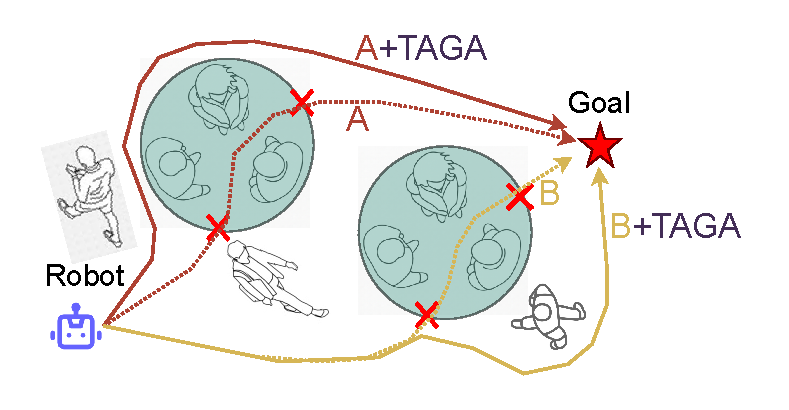
\includegraphics[width=4in]{figures/ntheme.pdf}
\vspace{-23pt}
 
\caption{Comparison of baseline and TAGA (group-aware) robot navigation in a multi-group environment. The \textcolor{blue}{robot} navigates toward the goal \textcolor{red}{$\bigstar$} through human groups (\textcolor[HTML]{70B0A8}{teal circles}) and individuals. Baseline navigation methods \textcolor[HTML]{AE4132}{A} and \textcolor[HTML]{D6B656}{B} (dotted lines) cut directly through group spaces, violating social norms (marked by \textcolor{red}{×}). In contrast, TAGA-enhanced paths \textcolor[HTML]{AE4132}{A}+TAGA and \textcolor[HTML]{D6B656}{B}+TAGA (solid lines) guide the robot around groups, respecting group boundaries while efficiently reaching the goal. \SR{I changed the caption. Some points were not clear in the previous one. Feel free to revise this one if required.}}
\vspace{-15pt} 
\label{fig-env-theme}
\end{figure}

% \caption{Comparison of baseline and TAGA (group-aware) robot navigation in a multi-group environment. The robot (blue icon, left) navigates toward its goal (red star, right) through a scene with two human groups (\textcolor[HTML]{70B0A8}{teal circles}) and several individuals (gray figures). Baseline navigation methods \textcolor[HTML]{AE4132}{A} and \textcolor[HTML]{D6B656}{B} (shown as dotted lines) cut directly through group spaces, violating social norms (marked by \textcolor{red}{×}). In contrast, TAGA-enhanced paths \textcolor[HTML]{AE4132}{A}+TAGA and \textcolor[HTML]{D6B656}{B}+TAGA (solid lines) guide the robot around groups, respecting group boundaries while efficiently reaching the goal.   \SR{I changed the caption. Some points were not clear in the previous one. Feel free to revise this as well.}}

% 

% \begin{figure}[!t]
% \centering
% 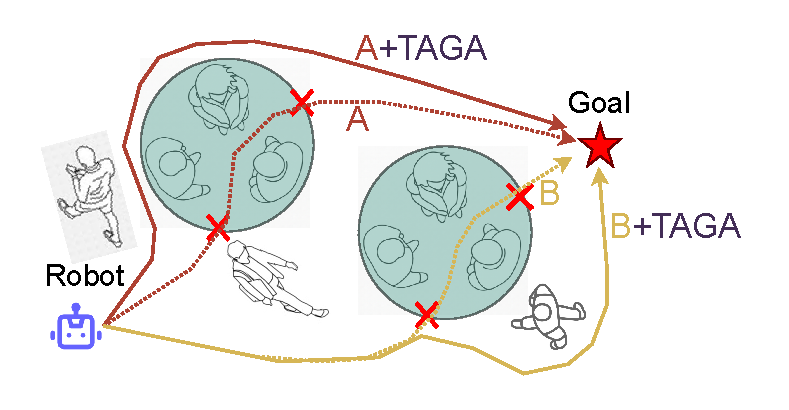
\includegraphics[width=4in]{figures/ntheme.pdf}
% \vspace{-23pt}
% \caption{
% % Comparison of robot navigation with and without TAGA integration. (a) Traditional environment without group modeling, where robots navigate toward goals without considering human group formations. (b) Our enhanced environment with detected human groups (bounded by dotted black circles). Existing navigation frameworks (labeled A and B) frequently intrude into these groups, while their TAGA-enhanced versions (A+TAGA and B+TAGA) generate paths that respect group boundaries while maintaining effective navigation toward goals. 

% % Comparison of baseline and TAGA (group-aware) paths in a multi-group environment. 
% % Baseline paths of \textcolor[HTML]{AE4132}{A} and \textcolor[HTML]{D6B656}{B} (shown as dotted lines) occasionally cross group boundaries, indicating violations of group constraints (highlighted by small `\textcolor{red}{×}' markers). In contrast, TAGA paths (\textcolor[HTML]{AE4132}{A}+TAGA and \textcolor[HTML]{D6B656}{B}+TAGA) remain fully within their assigned regions, demonstrating improved group compliance and cooperative navigation.

% Comparison of baseline and TAGA (group-aware) robot navigation in a multi-group environment. The robot (blue icon, left) navigates toward its goal (red star, right) through a scene with two human groups (\textcolor[HTML]{B0D1CB}{teal circles}) and several individuals (gray figures). Baseline navigation methods \textcolor[HTML]{AE4132}{A} and \textcolor[HTML]{D6B656}{B} (shown as dotted lines) cut directly through group spaces, violating social norms (marked by \textcolor{red}{×}). In contrast, TAGA-enhanced paths \textcolor[HTML]{AE4132}{A}+TAGA and \textcolor[HTML]{D6B656}{B}+TAGA (solid lines) guide the robot around groups, respecting group boundaries while efficiently reaching the goal.

% % \SR{The current two-panel design may confuse the reviewers. Panels (a) and (b) show different spatial arrangements of humans, which undermines the comparative purpose of the figure. Instead, redesign this as a single panel showing:
% % One environment with detected human groups (visualized with shaded regions or dotted boundaries)
% % Path A (group-unaware) - clearly intruding through groups,
% % Path B (group-unaware) - clearly intruding through groups,
% % Path A+TAGA (group-aware) - avoiding/respecting group boundaries, and
% % Path B+TAGA (group-aware) - avoiding/respecting group boundaries.
% % Use different colors and distinct line styles for each path with a clear legend. Make it visually obvious where group-unaware paths violate social norms - show paths cutting through group centers, contrasted with TAGA paths navigating around them.}
% } 
% % \SR{I think it's okay now. Consider adding small "×" markers where baseline paths intersect group boundaries to make violations more obvious. Write a good caption for the figure.\UT{Did it}}
% \vspace{-15pt} 
% \label{fig-env-theme}
% \end{figure}

Human crowds naturally organize into groups—families walking together, friends in conversation, colleagues moving between meetings—that create distinct spatial and social patterns \cite{moussaid2010walking}. These group formations significantly influence crowd flow and establish implicit boundaries that should be respected during navigation. When robots fail to recognize these group structures, they exhibit behaviors that humans perceive as rude or unsafe, such as cutting between conversing friends or passing through family clusters. Traditional navigation methods, including reactive approaches like Optimal Reciprocal Collision Avoidance (ORCA) \cite{orca} and Social Force models \cite{helbing1995social}, as well as learning-based systems \cite{liu2020decentralized, liu2023intention}, treat each person independently. Consequently, robots using these methods may achieve collision-free navigation while still violating social expectations by intruding into group spaces. Such violations induce psychological discomfort and stress in humans even when no physical danger is present, directly impacting human acceptance and willingness to share spaces with robots~\cite{gao2022evaluation}.

% \SR{The third paragraph (Recent attempts to....) needs revision to provide a comprehensive overview of related work. A strong introduction paragraph on prior work should: (1) introduce multiple relevant prior works on group-aware navigation, (2) systematically identify their limitations, and (3) complete the thought about the critical gap in real-time group detection. Currently, you cite only [11], which makes the literature review appear thin and incomplete. You have cited several other relevant group-aware methods in Section III—some of these should be briefly introduced here to demonstrate breadth of understanding.}

% \SR{Why completing the real-time group detection gap is essential:
% Your work makes a fundamental claim: TAGA uses DBSCAN for real-time group detection from observable features rather than assuming pre-labeled group membership. However, if you don't explicitly establish that existing methods assume perfect group knowledge and that this is a critical flaw, reviewers won't understand why your detection approach is a contribution. They'll wonder: "Why not just use ground-truth labels like prior work?"}

% Recent attempts to incorporate group awareness into robot navigation have shown promise but remain limited in scope. Katyal et al. \cite{group-aware} introduced group modeling using convex hulls, treating groups as unified entities moving in consistent directions. However, this approach struggles with the diversity of real-world group behaviors—static conversation circles, dynamically forming clusters, and groups with varying internal structures. Furthermore, their method relies on reinforcement learning with group-specific penalties, requiring retraining for different environments and lacking the flexibility to integrate with existing navigation systems. 

% \SR{Check the following revised para}

Recent attempts to incorporate group awareness into robot navigation have shown promise but face significant limitations. Katyal et al.~\cite{group-aware} introduced group modeling using convex hulls, treating groups as unified entities moving in consistent directions. However, this approach struggles with diverse real-world scenarios—such as static conversation circles, dynamically splitting clusters, and groups with non-uniform velocities. Their reinforcement learning approach with group-specific penalties requires retraining for different environments and cannot easily integrate with existing navigation systems. Similarly, geometric approaches like SEAN 2.0~\cite{tsoi2023sean} model F-formations with predefined spatial zones but require rigid formation parameters that don't adapt to dynamic group changes, while learning-based methods like SNGNN~\cite{wang2023learning} and CoMet~\cite{nishimura2022comet} need extensive training on group-labeled datasets.

% Most critically, current approaches often assume perfect knowledge of group membership, rather than addressing the challenge of real-time group detection in dynamic crowds.



\UT{Try to address the 1st review of reviwer 31281}Most critically, current approaches often assume perfect knowledge of group membership, rather than addressing the challenge of real-time group detection in dynamic crowds. In practical robot deployments, group membership is not observable---robots can only perceive individual positions and velocities through their sensors. They must infer group structure dynamically as people cluster, split, and reform. \SR{For instance, in Figure~\ref{fig-env-theme}, our proposed system intelligently distinguishes between an individual whose velocity is diverging from a nearby group (the person near the left group, moving away from it) versus an individual whose velocity is converging with a group (the person near the right group, moving toward it). In the former case, TAGA allows passage between the individual and group; in the latter, it treats them as a collective unit to navigate around.} Methods like~\cite{group-aware} that rely on pre-labeled group information or~\cite{tsoi2023sean} that require predefined F-formation parameters sidestep this fundamental challenge, limiting their applicability in real-world scenarios where group composition changes continuously.


% Most critically, current approaches often assume perfect knowledge of group membership, rather than addressing the challenge of real-time group detection in dynamic crowds. In practical robot deployments, group membership is not observable---robots can only perceive individual positions and velocities through their sensors. They must infer group structure dynamically as people cluster, split, and reform (Figure~\ref{fig-env-theme}). \SR{Our proposed system addresses this by using observable motion cues---detecting whether individuals' velocities are diverging from or converging toward nearby groups---to make real-time group membership decisions.} Methods like~\cite{group-aware} that rely on pre-labeled group information or~\cite{tsoi2023sean} that require predefined F-formation parameters sidestep this fundamental challenge, limiting their applicability in real-world scenarios where group composition changes continuously.

% To address these limitations, we present a comprehensive framework for group-aware robot navigation that combines realistic group modeling with a modular avoidance strategy. 
% % Building upon the simulation environment from \cite{liu2023intention}, we introduce dynamic group behaviors including spatial clustering, leader-follower dynamics, and varying group formations.
% \SR{We evaluate our approach in an extended simulation environment based on \cite{liu2023intention} }that incorporates dynamic group behaviors including spatial clustering, leader-follower dynamics, and varying group formations. Our key contribution is TAGA (Tangent Action for Group Avoidance), a reactive navigation module that computes tangent trajectories around detected groups. Unlike previous learning-based approaches, TAGA operates as a plug-in enhancement that can augment any existing navigation method without retraining, activating only when groups are detected and seamlessly returning control to the base navigation policy afterward. \SR{ As illustrated in Figure~\ref{fig-env-theme}, baseline paths cut through group spaces while TAGA paths respect group boundaries through tangent navigation.}


\SR{Building on this dynamic detection capability, we present} TAGA (Tangent Action for Group Avoidance), a comprehensive framework for group-aware robot navigation that combines realistic group modeling with a modular avoidance strategy. \SR{We evaluate our approach in an extended simulation environment based on~\cite{liu2023intention}} that incorporates dynamic group behaviors including spatial clustering, leader-follower dynamics, and varying group formations. Unlike previous learning-based approaches, TAGA operates as a plug-in enhancement that can augment any existing navigation method without retraining, activating only when groups are detected and seamlessly returning control to the base navigation policy afterward. \SR{As illustrated in Figure~\ref{fig-env-theme}, baseline paths cut through group spaces, while TAGA paths respect group boundaries through tangent navigation.}

% Our study makes the following contributions:
% \begin{enumerate}
%     \item We develop an enhanced simulation framework that models both individual and group dynamics with realistic clustering behaviors, leader-follower patterns, and mixed crowd compositions, enabling comprehensive evaluation of navigation strategies in complex social environments.
    
%     \item We propose TAGA, a modular group avoidance mechanism that dynamically computes tangent trajectories around detected human groups. TAGA integrates with existing navigation frameworks without requiring modification or retraining, demonstrating consistent improvements across reactive and learning-based methods.
    
%     \item We introduce Group Collision Rate (GCR) as an independent evaluation metric that measures the percentage of time robots spend within group boundaries. GCR provides continuous assessment of group-aware behavior throughout navigation episodes, where the traditional metrics satisfy SR + CR + TR = 1 for terminal states only. \SR{The current phrasing—"independent evaluation metric" and "where the traditional metrics satisfy SR + CR + TR = 1 for terminal states only"—is confusing and suggests GCR is superior to or separate from traditional metrics, when in fact it's complementary. Readers may misinterpret "independent" as meaning GCR doesn't relate to navigation quality, or that traditional metrics are flawed for only working at terminal states.}

%     \item \SR{We introduce Group Collision Rate (GCR) as a continuous metric complementary to traditional terminal state metrics. GCR measures the percentage of navigation time spent within group boundaries and provides frame-by-frame assessment of social compliance throughout the entire navigation episode. Unlike SR (?), CR(?), and TR(?) that only capture episode outcomes, GCR enables fine-grained evaluation of group-aware behavior.}
    
%     \item We implement a hierarchical safety controller that ensures individual collision avoidance during group maneuvers, addressing critical safety concerns when navigating near both groups and individuals simultaneously. This controller maintains multiple safety zones with graduated responses to prevent collisions while executing tangent trajectories.
    
%     \item We conduct comprehensive benchmarking across diverse scenarios including dense groups, mixed populations (50\% individuals, 50\% in groups), and dynamic formations. By integrating TAGA with established methods including ORCA \cite{orca}, Social Force \cite{helbing1995social}, DS-RNN \cite{liu2020decentralized}, and AG-RL \cite{liu2023intention}, we demonstrate \UT{I will give numbers later}
%     reduction in group intrusions while maintaining or improving navigation success rates.
% \end{enumerate}


Our study makes the following key contributions:

\begin{enumerate}
    \item \textbf{Real-time group detection.}
    We develop a DBSCAN-based module that identifies human groups online from observable motion cues (position, velocity, proximity), without assuming pre-labeled group membership.
    The module dynamically detects, updates, and dissolves group formations as they evolve, addressing a fundamental gap in practical socially compliant navigation.

    \item \textbf{Group-aware tangent navigation (TAGA).}
    We propose TAGA, a modular group-avoidance mechanism that computes tangent trajectories around detected group boundaries while maintaining individual safety.
    TAGA integrates with existing reactive and learning-based navigation frameworks without retraining, acting as a plug-in layer that activates only when groups are present.

    \item \textbf{Hierarchical safety control.}
    We design a three-zone safety controller (critical, warning, comfort) that coordinates group-level tangent maneuvers with individual collision avoidance in dense, mixed-population scenarios.

    \item \textbf{Realistic crowd simulation benchmark.}
    We introduce a benchmark environment incorporating five empirically motivated modeling phases: individual speed variation (Weidmann 1992), dynamic group speed coupling (Moussaïd 2010), F-formations for static groups (Kendon 1990), leader--follower dynamics (Helbing \& Molnár 1995), and convex-hull group boundaries.
    This benchmark enables reproducible evaluation under crowd conditions that closely reflect real-world group behavior.

    \item \textbf{Continuous group compliance metric (GCR).}
    We introduce the \textit{Group Collision Rate (GCR)}, a continuous metric that quantifies the fraction of navigation time spent inside group boundaries, providing frame-level social compliance assessment complementary to terminal-state metrics (SR, CR, TR).

    \item \textbf{Cross-method empirical study revealing reactive--learning asymmetry.}
    We benchmark TAGA against reactive methods (ORCA~\cite{orca}, Social Force~\cite{helbing1995social}) and learning-based methods (DS-RNN~\cite{liu2020decentralized}, AG-RL~\cite{liu2023intention}, GARN), uncovering a consistent pattern: explicit group-awareness yields the largest gains for reactive methods, while highly optimized learned policies that have implicitly internalized group-avoidance behavior benefit less.
    This finding offers concrete guidance on when modular group-awareness provides the most practical value.
\end{enumerate}

% \section{INTRODUCTION}

% \SR{Autonomous robots are rapidly transitioning from controlled industrial settings to complex human-populated environments—hospitals, shopping malls, airports, office buildings, and public spaces—where they must navigate alongside people to perform service tasks, deliveries, and assistance. Despite decades of research and significant technological progress, fundamental challenges still prohibit the seamless deployment of autonomous robots in crowded public environments~\cite{mavrogiannis2023core}. The consequences of poor social navigation extend beyond inefficiency: robots' navigational behaviors—such as how they approach and pass people—can induce feelings of discomfort or stress in humans, even when they don't physically endanger anyone. Field deployments in shopping malls have documented failed robot approaches and highlighted the need for socially acceptable navigation when interacting with the public. Studies measuring human comfort show that participants rate their psychological comfort significantly lower under various robot approach patterns and speeds~\cite{gao2022evaluation}. These failures directly impact human acceptance and willingness to share spaces with robots—a critical barrier as society increasingly relies on robotic systems for essential services. As robots become more prevalent in our daily lives, developing navigation strategies that not only avoid collisions but actively respect human social norms has emerged as an essential requirement for successful human-robot coexistence.}

% Autonomous robots are increasingly being used in human environments for various applications, including service robotics, delivery, and assistive technologies. A growing number of research has focused on developing human-aware robot navigation by accounting for the fast and dynamic nature of human motion while adhering to complex social norms \cite{CHARALAMPOUS201785, pandey2017mobile}. \UT{Socially compliant navigation refers to the robot's ability to navigate in a manner that respects human social interactions and follows socially accepted norms and behaviors in a given environment.}  
% \SR{Early approaches to achieving social compliance evolved from simply treating humans as moving obstacles to avoid \cite{fox1997dynamic}, to designing strategies to prevent robots from getting stuck in crowds \cite{trautman2015robot}, and eventually incorporating basic social norms to enable more appropriate navigation behaviors \cite{bera2017sociosense}.}
% % Early studies approached this problem by treating humans as moving obstacles to avoid \cite{fox1997dynamic}, designing strategies to prevent robots from getting stuck in crowds \cite{trautman2015robot}, and incorporating social norms to enable socially appropriate navigation \cite{bera2017sociosense}. 
% % and incorporating social norms to enable socially appropriate navigation \cite{bera2017sociosense}. 
% However, most of these methods have modeled humans as independent individuals without considering the impact of groups on navigation.
% % rios2015proxemics, , KRUSE20131726
% % , robicquet2016learning
% \begin{figure}[!t]
% \centering
% 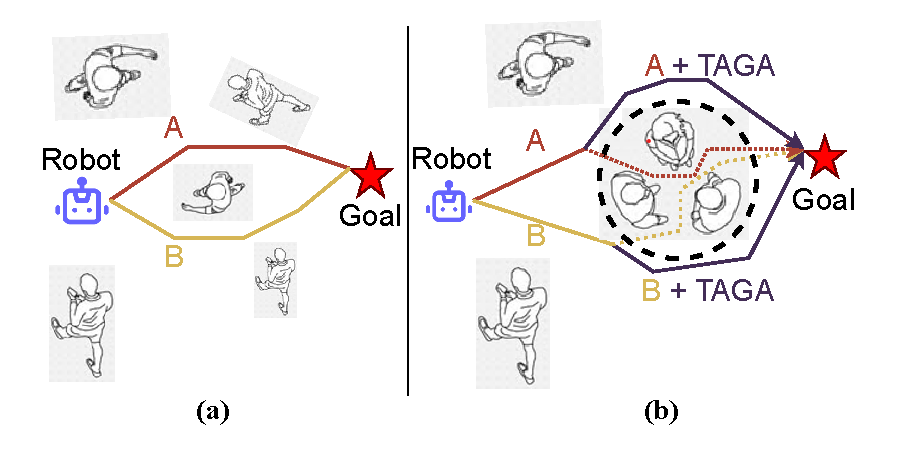
\includegraphics[width=4in]{figures/theme.pdf}
% \vspace{-23pt}
% \caption{\SR{Comparison of robot navigation with and without TAGA integration. (a) Traditional environment without group modeling, where robots navigate toward goals without considering human group formations. (b) Our enhanced environment with human groups (bounded by dotted black circles). Existing navigation frameworks (labeled A and B) frequently intrude into these groups, while their TAGA-enhanced versions (A+TAGA and B+TAGA) generate paths that respect group boundaries while maintaining effective navigation toward goals.}
% % (a) The figure represents the previous existing environment, which does not include human groups or defined boundaries. (b) In contrast, our modified environment introduces extended human groups, with group boundaries indicated by dotted black circles. Existing navigation frameworks like A and B struggle to adapt to group behaviors and often cross these boundaries. However, when our modular TAGA model is integrated with A and B, it effectively adapts to group behaviors, enabling appropriate interactions and crossings while respecting group boundaries.
% }
% The modified simulation environment used in this study. The figure shows a robot navigating towards a goal while predicting human positions. Humans within the robot’s observation area influence its trajectory, whereas those outside do not. The model considers both individual humans and human groups for socially aware navigation.
% \vspace{-15pt} 
% \label{fig-env-theme}
% \end{figure}

% In real-world crowded environments, people naturally form dynamic groups that move together, interact, and collectively influence navigation patterns \cite{moussaid2010walking}. Traditional approaches, such as reaction-based methods like Optimal Reciprocal Collision Avoidance (ORCA) \cite{orca} and Social Force (SF) \cite{helbing1995social}, as well as learning-based models \cite{liu2020decentralized, liu2023intention}, generally treat humans as separate individuals, failing to capture group-level interactions. As a result, robots relying on these methods may exhibit inefficient or socially inappropriate behaviors, such as cutting through groups rather than respecting their collective behaviors.

% Recently, a study \cite{group-aware} attempted to address this issue by introducing a group-aware policy for robot navigation, representing human groups using convex hulls and modeling them as pedestrians moving in the same direction. While their approach improves social compliance by discouraging the robot from intruding into groups, it lacks adaptability in mixed environments, as it primarily focuses on groups while overlooking individual interactions and more structured formations, such as static groups. 

% To overcome these limitations, we introduce human group modeling within a robot navigation framework utilizing the simulation environment from \cite{liu2023intention}, enabling robots to interact with both individual humans and human group behaviors (See Fig. \ref{fig-env-theme}). Additionally, we propose Tangent Action for Group Avoidance (TAGA), a reactive group-aware navigation model that dynamically adjusts robot trajectories based on detected human groups. Unlike previous approaches that rely solely on learned policies, TAGA provides a flexible avoidance mechanism that can be integrated into existing navigation methods, allowing these methods to adapt to group behaviors when human groups are present.

%To systematically evaluate the effectiveness of our approach, we conducted extensive experiments in diverse crowd settings. 
% Our study makes the following contributions:

% \begin{enumerate}
%     \item We developed an enhanced simulation framework that models both individual human dynamics and group behaviors with spatial clustering and leader-follower dynamics. This environment enables the evaluation of navigation strategies in complex crowd scenarios with diverse group formations.
    
    
%     % \item We developed an enhanced simulation framework that realistically models both individual human dynamics and human group behaviors, incorporating spatial clustering, leader-follower dynamics, and group boundary recognition. This environment enables the systematic evaluation of navigation strategies in complex crowd scenarios with diverse group formations.
    
%     \item We proposed TAGA, a reactive-based group avoidance mechanism that can be integrated into any robot navigation framework, allowing robots to dynamically adapt to human group behaviors and navigate in a socially compliant manner.
    
%     \item We introduced a new evaluation metric, Group Collision Rate (GCR), which quantifies how well a robot avoids intruding into human groups, providing a standardized approach to measure group-aware navigation performance.
    
%     \item We conducted a comprehensive benchmarking study by integrating TAGA with existing methods, including ORCA \cite{orca}, SF \cite{helbing1995social}, DS-RNN \cite{liu2020decentralized}, and AG-RL \cite{liu2023intention}, demonstrating significant improvements in group-aware navigation while maintaining comparable performance in other metrics.

%     \end{enumerate}

% \begin{enumerate}
%     \item \UT{We developed an advanced robot crowd interaction simulation environment that not only allows for the interaction of individual humans with the robot but also models dynamic human groups, providing a more realistic and comprehensive platform for evaluating navigation strategies in complex crowd scenarios.}
%     \item  We proposed a reactive-based group avoidance mechanism that can be integrated into any robot navigation framework, allowing robots to dynamically adapt to human group behaviors and navigate in a socially compliant manner.
%     \item To evaluate our model, we conducted a comprehensive benchmarking study by integrating TAGA with existing methods, including ORCA \cite{orca}, Social Force (SF) \cite{helbing1995social}, Decentralized Structural-RNN (DS-RNN) \cite{liu2020decentralized}, and Attention-Graph RL  (AG-RL) \cite{liu2023intention} Navigation models, to assess its impact on navigation performance. Additionally, to quantify group-aware navigation performance, we introduced a new evaluation metric, Group Collision Rate (GCR), which measures how well a robot avoids intruding into human groups.
% \end{enumerate}
% 1) We developed a robot crowd interaction simulation environment, where both individual humans and human groups can interact with the robot. This environment enables evaluating navigation strategies in realistic crowd scenarios.  
% 2) We proposed a reactive-based group avoidance mechanism that can be integrated into any robot navigation framework, allowing robots to dynamically adapt to human group behaviors and navigate in a socially compliant manner.  
% 3) To evaluate our model, we conducted a comprehensive benchmarking study by integrating TAGA with existing methods, including ORCA \cite{orca}, Social Force (SF) \cite{helbing1995social}, Decentralized Structural-RNN (DS-RNN) \cite{liu2020decentralized}, and Attention-Graph RL  (AG-RL) \cite{liu2023intention} Navigation models, to assess its impact on navigation performance. Additionally, to quantify group-aware navigation performance, we introduced a new evaluation metric, Group Collision Rate (GCR), which measures how well a robot avoids intruding into human groups.  


% Autonomous robots are increasingly being used in human environments for various applications, including service robotics, delivery, and assistive technologies. A growing number of research has focused on developing human-aware robot navigation by accounting for the fast and dynamic nature of human motion while adhering to complex social norms \cite{CHARALAMPOUS201785, pandey2017mobile, KRUSE20131726}. Early studies approached this problem by treating humans as moving obstacles to avoid \cite{fox1997dynamic}, designing strategies to prevent robots from getting stuck in crowds \cite{trautman2015robot}, and incorporating social norms to enable socially appropriate navigation \cite{robicquet2016learning, bera2017sociosense}. However, most of these methods have modeled humans as independent individuals, without considering the impact of groups on navigation.

% In real-world crowded environments, people naturally form dynamic groups that move together, interact, and collectively influence navigation patterns. Traditional approaches, such as reaction-based methods like Optimal Reciprocal Collision Avoidance (ORCA) \cite{orca} and Social Force (SF) \cite{helbing1995social}, as well as learning-based models \cite{liu2020decentralized, liu2023intention}, generally treat humans as separate individuals, failing to capture group-level interactions. As a result, robots relying on these methods may exhibit inefficient or socially inappropriate behaviors, such as cutting through groups rather than respecting their collective behaviors.

% Recently, a study \cite{group-aware} addressed this issues and introduced a group-aware policy for robot navigation by representing human groups using convex hulls and modeling them as pedestrians moving in the same direction. While their approach improves social compliance by discouraging the robot from intruding into groups, it lacks adaptability in mixed environments, as it primarily focuses on groups while overlooking individual interactions and more structured formations, such as static groups. 
% % Furthermore, their method relies solely on a learned policy, limiting real-time adaptability in complex scenarios.

% In this study, we address these limitations by introducing human group modeling within a robot navigation framework utilizing the simulation environment from \cite{liu2023intention}, enabling robots to interact with both individual humans and human group behaviors. Additionally, we propose TAGA, a reactive group-aware navigation model that dynamically adjusts robot trajectories based on detected human groups. TAGA provides a flexible avoidance mechanism that can be integrated into existing navigation approaches, allowing these methods to adapt to human group behaviors when a human group is detected.

% In this study, we address these limitations by introducing human group modeling within a robot navigation framework utilizing the simulation environment from \cite{liu2023intention}, enabling robots to interact with both individual humans and human groups. Additionally, we propose TAGA, a reactive group-aware navigation model that dynamically adjusts robot trajectories based on detected human groups. TAGA provides a flexible avoidance mechanism that can be integrated into existing navigation approaches, allowing these methods to adapt to group behaviors when human groups are present.

% Our study makes the following contributions.  
% 1) We developed a robot crowd interaction simulation environment, where both individual humans and human groups can interact with the robot. This environment enables evaluating navigation strategies in realistic crowd scenarios.  
% 2) We proposed a reactive-based group avoidance mechanism that can be integrated into any robot navigation framework, allowing robots to dynamically adapt to human group behaviors and navigate in a socially compliant manner.  
% 3) To evaluate our model, we conducted a comprehensive benchmarking study against ORCA \cite{orca}, Social Force (SF) \cite{helbing1995social}, DS-RNN \cite{liu2020decentralized}, and Intention-Aware Navigation (IAN) \cite{liu2023intention}. Additionally, to quantify group-aware navigation performance, we introduced a new evaluation metric, Group Collision Rate (GCR), which measures how well a robot avoids intruding into human groups.
% Unlike previous approaches that rely purely on learned policies, TAGA integrates a tangent-based avoidance mechanism, allowing real-time adaptability. 
% Furthermore, we introduce a new performance metric, Group Collision Rate (GCR), to quantitatively assess how well a robot avoids intruding into human groups.


% To evaluate our approach, we conduct a comprehensive benchmarking study against widely used navigation models, including ORCA \cite{orca}, SF \cite{helbing1995social}, DS-RNN \cite{liu2020decentralized}, and Intention-Aware Navigation (IAN) \cite{liu2023intention}. These methods primarily focus on individual human interactions, lacking explicit mechanisms for handling groups. By extending their frameworks to incorporate human group modeling, we assess their effectiveness in dense social settings. Our results demonstrate that TAGA significantly reduces group intrusions while maintaining competitive navigation efficiency compared to state-of-the-art baselines.
% Our study makes the following contributions.  
% 1) We developed a robot crowd interaction simulation environment, where both individual humans and human groups can interact with the robot. This environment enables evaluating navigation strategies in realistic crowd scenarios.  
% 2) We proposed a reactive-based group avoidance mechanism that can be integrated into any robot navigation framework, allowing robots to dynamically adapt to human group behaviors and navigate in a socially compliant manner.  
% 3) To evaluate our model, we conducted a comprehensive benchmarking study against ORCA \cite{orca}, Social Force (SF) \cite{helbing1995social}, DS-RNN \cite{liu2020decentralized}, and Intention-Aware Navigation (IAN) \cite{liu2023intention}. Additionally, to quantify group-aware navigation performance, we introduced a new evaluation metric, Group Collision Rate (GCR), which measures how well a robot avoids intruding into human groups.






% This template provides authors with most of the formatting specifications needed for preparing electronic versions of their papers. All standard paper components have been specified for three reasons: (1) ease of use when formatting individual papers, (2) automatic compliance to electronic requirements that facilitate the concurrent or later production of electronic products, and (3) conformity of style throughout a conference proceedings. Margins, column widths, line spacing, and type styles are built-in; examples of the type styles are provided throughout this document and are identified in italic type, within parentheses, following the example. Some components, such as multi-leveled equations, graphics, and tables are not prescribed, although the various table text styles are provided. The formatter will need to create these components, incorporating the applicable criteria that follow \cite{liu2020decentralized, liu2023intention}






\section{BACKGROUND AND RELATED WORK}

\subsection{Human Group Modeling in Crowd-Robot Simulation Frameworks}

Recent studies have expanded human-aware robot navigation to account for both static and dynamic social groups \cite{group-aware}, where static groups are defined as individuals who stay spatially close with minimal movement, while dynamic groups move together toward a common goal. Prior research has explored group interactions based on size and formation \cite{kato2015may} and investigated intra-group coherence \cite{luber2013multi,taylor2020robot} and inter-group differences \cite{shao2014scene} to improve trajectory prediction \cite{unhelkar2015human}. However, these approaches typically require explicit group structure definitions or extensive training data, limiting their adaptability to diverse real-world scenarios.

Machine learning has significantly advanced human-aware robot navigation. RNNs \cite{alahi2016social} have been used for human motion prediction \cite{bisagno2018group}, while RL methods, including inverse RL \cite{kretzschmar2016socially} and DRL \cite{chen2019relational}, have improved socially compliant navigation. Attention-based DRL has further enhanced interaction modeling in crowded settings \cite{chen2019crowd,chen2017decentralized}. However, these learning-based approaches suffer from three critical limitations: (1) they require extensive retraining when group dynamics change, (2) they cannot easily integrate with existing navigation systems, and (3) they typically assume perfect group membership knowledge rather than addressing real-time detection challenges \cite{gao2022evaluation}.

% \SR{(}
% A recent work \cite{group-aware} addressed group modeling using convex hulls for group representation, but their approach relies on reinforcement learning penalties and assumes groups move uniformly in the same direction. This limits adaptability to real-world scenarios where groups exhibit diverse behaviors—static conversation circles, dynamically splitting clusters, or mixed formations with varying velocities. Additionally, their evaluation metric treats group collisions as terminal states, preventing nuanced assessment of navigation quality.\SR{)} \SR{You already discussed \cite{group-aware} extensively in the introduction. This feels repetitive. Add new technical details not mentioned in intro (e.g., specific network architecture, reward formulation, training requirements)}

% Done by uk
Recently, Katyal \textit{et al.}~\cite{group-aware} introduced a reinforcement learning framework that models group boundaries as convex hulls and penalizes intrusions through a custom reward function integrated into a PPO-based navigation policy. 
While effective under static group structures, their model assumes uniform group motion and requires retraining to adapt to new group configurations, limiting its deployment in dynamic crowds.
% Done by maam
To address these fundamental limitations in group detection, modeling flexibility, and evaluation, we develop TAGA as a modular enhancement compatible with diverse navigation methods, as detailed in Section~\ref{sec:methods}.
% \SR{(}In contrast to these limitations, we present three key innovations. First, leveraging the framework from \cite{liu2023intention}, we create a simulation environment that models realistic group behaviors including leader-follower dynamics, dynamic formation changes, and mixed static-dynamic groups. Second, unlike learning-based methods that require retraining, our TAGA mechanism operates as a modular plug-in that enhances any existing navigation method without modification. Third, we introduce GCR as a continuous metric measuring the percentage of time spent in group spaces, providing more granular evaluation than binary collision states. \SR{)} \SR{Highly repetitive to your contribution list. Better exclude this paragraph.}



\subsection{Navigation Methods for Human Group Avoidance}

Robot navigation in crowded environments has evolved through two primary paradigms: reaction-based and learning-based methods. Reaction-based models like ORCA \cite{orca} and Social Force \cite{helbing1995social} use mathematical formulations for collision avoidance. ORCA computes velocity obstacles for guaranteed collision-free paths but treats all agents equally, leading to socially inappropriate behaviors like cutting through groups. The Social Force model incorporates attractive and repulsive forces \cite{ferrer2013robot} but struggles with parameter tuning for different group densities and formations. Extended Social Force variants \cite{zanlungo2011social} have attempted to model group coherence, but remain limited to predefined group structures.

Learning-based approaches have shown promise in capturing complex crowd dynamics. DS-RNN \cite{liu2020decentralized} uses structural-RNN to model spatio-temporal relationships, while AG-RL \cite{liu2023intention} employs attention mechanisms for intention prediction. SARL \cite{chen2019crowd} introduces social attention for multi-agent interactions, and recent graph neural network approaches \cite{wang2023learning} model relational structures in crowds. However, these methods fundamentally treat humans as individuals with pairwise interactions, lacking explicit group-level understanding.

Recent group-aware methods attempt to bridge this gap through various approaches. Wang et al. \cite{wang2023learning} propose SNGNN using graph neural networks to model group relationships, but require extensive training on group-specific datasets. Nishimura et al. \cite{nishimura2022comet} introduce CoMet, modeling group cohesion forces through learned parameters that must be tuned for different environments.
% Done by Ma'am
These training and tuning requirements limit rapid deployment across different venues (hospitals vs. malls vs. airports) where crowd dynamics vary significantly. % End here 
Bisagno et al. \cite{bisagno2018group} use LSTM networks for group trajectory prediction but focus on prediction rather than navigation. Geometric approaches like SEAN 2.0 \cite{tsoi2023sean} model F-formations with O-space, P-space, and R-space zones \cite{kendon1990conducting}, but require predefined spatial configurations that may not generalize to dynamic groups.

Our TAGA approach fundamentally differs from these methods in three ways. First, while existing methods require either extensive training (learning-based) or rigid geometric rules (zone-based), TAGA dynamically computes tangent trajectories based on real-time group detection without predefined parameters. Second, unlike methods that replace existing navigation systems, TAGA operates as a conditional module that activates only when groups are detected, preserving the original navigation performance for individual interactions. Third, TAGA's modular design allows integration with any navigation method—reactive or learned—without retraining, demonstrated through successful integration with ORCA, Social Force, DS-RNN, and AG-RL.

\subsection{Evaluation Metrics and Benchmarking}

Existing evaluation metrics for socially-aware navigation primarily focus on individual interactions. Success Rate (SR), Collision Rate (CR), and Timeout Rate (TR) measure terminal states \cite{gao2022evaluation}, while path efficiency and comfort distance assess trajectory quality \cite{mavrogiannis2023core}. For group-aware navigation, prior work \cite{group-aware} treats group collisions as terminal failures, conflating them with individual collisions and preventing nuanced evaluation of group interaction quality.

% Social compliance metrics have attempted to capture group awareness through indirect measures. Pedestrian discomfort \cite{trautman2015robot} estimates psychological comfort but lacks direct group boundary assessment. Personal space invasion metrics \cite{kirby2009companion} consider individual zones but not collective group spaces. The Social Individual Index \cite{truong2017toward} measures disruption to social conversations but requires knowing conversation states. \SR{This para sounds somewhat mechanical. You're  following a template of "Metric X does Y but lacks Z" three times in a row. While the critiques are valid, the paragraph would be stronger if you synthesized these limitations into a broader insight.}

% \SR{Check the following revised para. Feel free to modify.}
% Done by Ma'am
Existing social compliance metrics attempt to capture group awareness through indirect measures such as pedestrian discomfort~\cite{trautman2015robot}, personal space invasion~\cite{kirby2009companion}, and conversation disruption~\cite{truong2017toward}. However, these approaches either rely on proxy measures like psychological comfort rather than direct spatial assessment, focus on individual rather than collective group zones, or require additional context such as conversation states that may not be observable. Consequently, they cannot directly quantify the core behavior of interest: the amount of time a robot spends occupying group spaces during navigation.
% We introduce Group Collision Rate (GCR) as an independent continuous metric that directly measures the percentage of navigation time spent within detected group boundaries. GCR provides granular assessment throughout episodes, enabling distinction between brief necessary intrusions and prolonged inappropriate occupancy of group spaces. This metric operates independently of terminal states (maintaining SR + CR + TR = 1) while providing actionable feedback for improving group-aware behaviors. Our comprehensive evaluation across diverse scenarios—dense groups, mixed populations (50\% grouped, 50\% individual), dynamic formations, and groups-only environments—demonstrates TAGA's consistent performance improvements across varying crowd compositions. \SR{This para on GCR also sounds repetitive. Rewrite.}
% Done by me
In all experiments, we report the Group Collision Rate (GCR) together with SR, CR, and TR as a continuous indicator of group intrusions during navigation.









% \section{BACKGROUND AND RELATED WORK}

% \subsection{Human Group Modeling in Crowd-Robot Simulation Frameworks}

% Recent studies have expanded human-aware robot navigation to account for both static and dynamic social groups \cite{group-aware}, where static groups are defined as individuals who stay spatially close with minimal movement, while dynamic groups move together toward a common goal. Prior research has explored group interactions based on size and formation \cite{kato2015may} and investigated intra-group coherence \cite{luber2013multi,taylor2020robot} and inter-group differences \cite{shao2014scene} to improve trajectory prediction \cite{unhelkar2015human}. However, dynamic groups often lack structured formations, requiring adaptive strategies for effective navigation.

% Machine learning has significantly advanced human-aware robot navigation. RNNs \cite{alahi2016social} have been used for human motion prediction \cite{bisagno2018group}, while RL methods, including inverse RL \cite{kretzschmar2016socially} and DRL \cite{chen2019relational}, have improved socially compliant navigation. Attention-based DRL has further enhanced interaction modeling in crowded settings \cite{chen2019crowd,chen2017decentralized}. However, most approaches focus on individual interactions, with limited emphasis on explicit group modeling \cite{gao2022evaluation}. A prior work \cite{group-aware} addressed this by using convex hulls instead of F-formations \cite{chen2019relational} for group representation, but it relies on predefined structures and RL-based penalties, making it less adaptable to dynamic environments. Additionally, it overlooks individual interactions and lacks a robust evaluation metric for group-aware navigation.

% In contrast, leveraging the framework from \cite{liu2023intention}, we integrated human groups alongside individual dynamic humans for a more realistic crowd simulation. To assess group-aware navigation, we compare our model with state-of-the-art frameworks. Existing metrics primarily penalize group intersections or measure pedestrian discomfort \cite{group-aware}, offering only indirect assessments of social compliance. To address this, we propose GCR, a more robust metric that directly quantifies a robot’s ability to avoid intruding into human groups, ensuring a precise and continuous evaluation across different models.

% % \vspace{-2pt}
% \subsection{Navigation Methods for Human Group Avoidance}

% Robot navigation in crowded environments requires safe and efficient interaction with both individuals and human groups. Traditional approaches fall into reaction-based and learning-based methods. Reaction-based models like ORCA \cite{orca} and SF \cite{helbing1995social} use predefined mathematical rules for collision avoidance. ORCA enables fast trajectory adjustments but ignores social norms, often leading to group intrusions. The SF Model incorporates interaction forces but struggles with dynamically changing groups. Overall, these methods lack the adaptability required for complex, human-centric environments.

% % Previously it was included
% Learning-based methods, including DS-RNN \cite{liu2020decentralized} and AG-RL \cite{liu2023intention}, leverage deep reinforcement learning to model crowd interactions. DS-RNN captures spatio-temporal relationships but focuses on individual-based interactions rather than structured group behaviors. AG-RL predicts human intentions using attention-based interaction graphs but does not explicitly differentiate human groups, leading to suboptimal group avoidance. To overcome this issue, a recent group-aware navigation model\cite{group-aware}, define groups using convex hulls and penalize group intrusions. However, they assume groups move in the same direction and lack adaptability for static or mixed groups. In contrast, our proposed TAGA navigation model can dynamically adjust robot trajectories based on detected human groups, whether they are static or mixed, and integrate with existing frameworks for improved navigation. 
% Learning-based methods, such as DS-RNN \cite{liu2020decentralized} and AG-RL \cite{liu2023intention}, utilize deep reinforcement learning to model crowd interactions. DS-RNN captures spatio-temporal relationships but focuses on individual interactions rather than structured group behaviors. AG-RL employs attention-based interaction graphs to predict human intentions but does not explicitly differentiate human groups, leading to suboptimal group avoidance. A recent group-aware approach \cite{group-aware} defines groups using convex hulls and penalizes intrusions but assumes groups move in the same direction, limiting adaptability for static or mixed groups. In contrast, our proposed TAGA model dynamically adjusts robot trajectories based on detected human groups, regardless of their movement patterns, while seamlessly integrating with existing frameworks for improved navigation.










% To address these limitations, we propose TAGA, a reactive group-aware navigation model that dynamically adjusts robot trajectories based on detected human groups. Unlike prior approaches, TAGA enables real-time adaptation, integrates with existing frameworks, and introduces Group Collision Rate (GCR) as a new evaluation metric to measure group intrusion performance.




% \subsection{Benchmarking Group-Aware Navigation and Evaluation Metrics}

% \textit{Recent group-aware navigation methods can be categorized into learning-based and geometric approaches. Wang et al. [2023] propose SNGNN, using graph neural networks to model group relationships but requiring extensive training. Nishimura et al. [2022] introduce CoMet, modeling group cohesion forces through learned parameters. Bisagno et al. [2021] use LSTM networks for group trajectory prediction. These methods require training on group-specific datasets and cannot be easily integrated with existing navigation systems.
% In contrast, geometric approaches like SEAN 2.0 [Tsoi et al., 2023] use F-formations for group representation but require predefined group structures. Our TAGA method differs by being modular, requiring no training, and capable of enhancing any existing navigation method with group awareness. We compare TAGA against two group-aware baselines: (1) Zone-based avoidance, which creates larger repulsive zones around detected groups, and (2) F-formation avoidance inspired by SEAN 2.0 [Tsoi et al., 2023], which models the O-space, P-space, and R-space of human group formations. Unlike these methods that use predefined geometric rules, TAGA dynamically computes tangent trajectories while maintaining modularity with existing navigation methods
% }
\section{TANGENT ACTION MODEL FOR GROUP AVOIDANCE}
\label{sec:methods}

\subsection{Problem Formulation and Group Detection}

Our objective is to enable a robot to navigate to its goal while respecting both individual humans and group formations in dynamic environments. We formulate this as a conditional decision problem where the robot adapts its behavior based on real-time detection of human groups.

\UT{Try to address the 4th review of reviwer 31289}Rather than assuming perfect group knowledge, we employ spatial clustering for real-time group detection. At each timestep, we identify groups using DBSCAN with adaptive parameters: proximity threshold $\epsilon = 1.5$m and minimum group size of 2. Groups are detected based on spatial proximity and velocity alignment:

\begin{equation}
G_j = \{h_i | d(h_i, h_k) < \epsilon, |\mathbf{v}_i - \mathbf{v}_k| < v_{thresh}, \forall h_k \in G_j\}
\end{equation}

where $d(h_i, h_k)$ is the Euclidean distance between humans and $v_{thresh}$ is the velocity difference threshold for cohesive movement.

The robot observes the environment state $s_t$ comprising robot features $w_t$ (position, velocity, goal), individual humans $\{u_i^t\}_{i=1}^n$, and detected groups $\{g_j^t\}_{j=1}^m$:

\begin{equation}
s_t = \{w_t, u_1^t, ..., u_n^t\} \cup \{g_1^t, ..., g_m^t\}
\end{equation}

Each detected group $g_j^t$ is characterized by its centroid $C$, radius $R$, and member count $m_g$, where $C = \frac{1}{|G_j|}\sum_{h_i \in G_j} p_i$ and $R = \max_{h_i \in G_j} ||p_i - C||$.

\begin{figure}[!t]
\centering
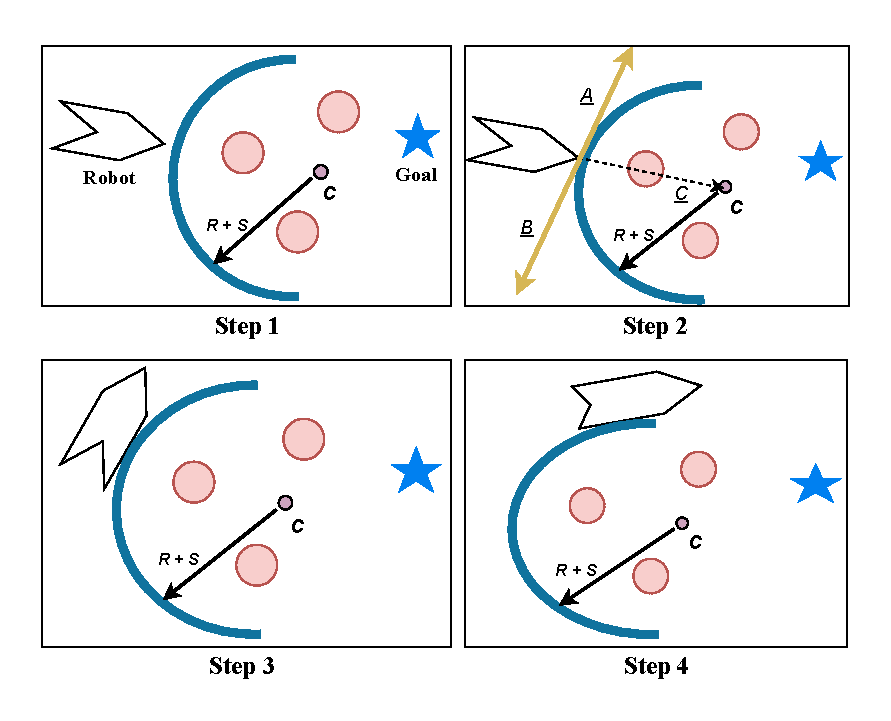
\includegraphics[width=3.5in]{figures/taga.pdf}
\caption{Visualization of the proposed TAGA process. The robot detects a human group with centroid $C$ and radius $R$. When the robot reaches switching distance $R+S$ from the centroid (where $S$ is the safety margin), TAGA activates and computes tangent trajectories. The robot navigates along the circular boundary at distance $R+S$ from $C$, selecting between clockwise and counterclockwise paths based on goal direction and safety constraints. Once past the group, TAGA deactivates and returns control to the baseline navigation policy.\UT{Step description require}}
\label{fig:taga-process}
\end{figure}

\subsection{Tangent-Based Navigation with Safety Guarantees}
\UT{Try to address the 3rd review of reviwer 31281 of safety concerns of individuals}
TAGA activates when the robot approaches a detected group within switching distance $R + S$ from the group centroid, where $R$ is the group radius and $S$ is a safety margin (typically 0.5m) beyond the group boundary. As illustrated in Figure \ref{fig:taga-process}, when $d(r, C) \leq R + S$, the robot computes a tangent trajectory that maintains this safe distance from the centroid. The tangent point on the circular boundary is:

\begin{equation}
p_T = C + (R + S) \cdot \hat{t}
\end{equation}

where $\hat{t}$ is the unit tangent vector. The robot selects between clockwise and counterclockwise tangent directions:

\begin{equation}
\hat{t} = \arg\min_{t \in \{t_{cw}, t_{ccw}\}} \left( w_1 \cdot \angle(t, \vec{g}) + w_2 \cdot d_{obs}(t) \right)
\end{equation}

where $\angle(t, \vec{g})$ measures angular deviation from the goal direction and $d_{obs}(t)$ accounts for obstacles along the tangent path.

To ensure individual collision avoidance during group maneuvers, we implement a hierarchical safety controller with graduated response zones:

\begin{equation}
a_{final} = \begin{cases}
    a_{stop} & d_{min} < d_{critical} \\
    \alpha a_{TAGA} + (1-\alpha) a_{avoid} & d_{critical} \leq d_{min} < d_{personal} \\
    a_{TAGA} & d_{min} \geq d_{personal}
\end{cases}
\end{equation}

where $d_{min} = \min_i d(r, h_i)$., $d_{critical} = 0.3$m triggers emergency stop, $d_{personal} = 0.5$m initiates blended avoidance, and:
\begin{equation}
\alpha = \frac{\min_i d(r, h_i) - d_{critical}}{d_{personal} - d_{critical}}
\end{equation}
provides smooth transitions between behaviors. This ensures that while navigating around groups at distance $R+S$, the robot maintains safe distances from any individuals who may be near but outside the detected group.

\subsection{Integration and Switching Mechanism}

\UT{Try to address the 2nd review of reviwer 31289}TAGA operates as a modular enhancement to existing navigation methods. Given a baseline navigation model $M$ (either reactive or learned), the integrated system follows:

\begin{equation}
\pi(s_t) = \begin{cases}
    \text{TAGA}(s_t) & \text{if group detected AND} \\
    & d(r, C) \leq R + S \text{ AND approaching} \\
    M(s_t) & \text{otherwise}
\end{cases}
\end{equation}

% The complete activation condition ensures TAGA engages only when necessary:

% \begin{equation}
% \text{activate} = (d(r, C) \leq R + S) \land (\vec{v}_r \cdot \vec{rC} > 0) 
% % \land (\text{conf} > \tau)
% \end{equation}

% where $\vec{v}_r$ is robot velocity, $\vec{rC}$ is the vector from robot to group centroid, and $\tau$ is the detection confidence threshold. The approaching condition $(\vec{v}_r \cdot \vec{rC} > 0)$ prevents unnecessary activation when moving away from groups.

% Deactivation occurs when the robot moves beyond $(R + S) + \delta$ from the centroid, where hysteresis margin $\delta = 0.2$m prevents oscillation between modes. The modular design preserves the baseline model's performance for individual interactions while adding group awareness without retraining. 

% Computational overhead remains minimal with $O(n \log n)$ for group detection and $O(k)$ for tangent computation across $k$ groups, enabling real-time operation at 10Hz. This integration approach allows TAGA to enhance any existing navigation framework—demonstrated through successful integration with ORCA, Social Force, DS-RNN, and AG-RL—while maintaining their original capabilities for scenarios without groups.

% \section{Tangent Action Model for Group Avoidance}

%  \begin{figure}[t]
%     \centering
%     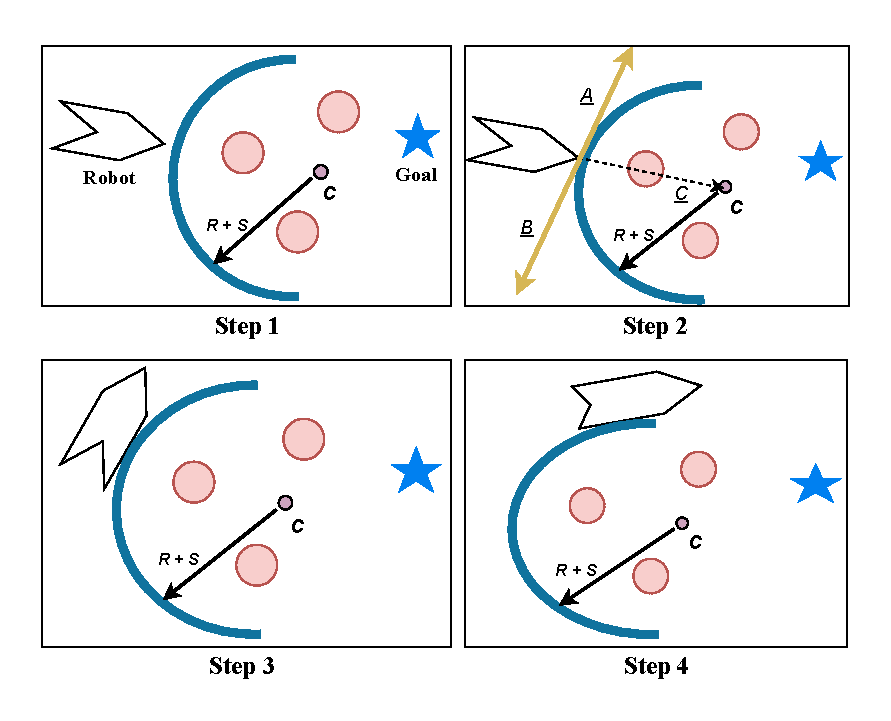
\includegraphics[scale=0.5]{figures/taga.pdf}
%     \caption{The Visualization of our proposed TAGA process. The robot, initially following a standard navigation model, detects a human group and activates TAGA. The model computes a tangent action based on the group centroid and boundary, enabling the robot to smoothly navigate around the group while ensuring social compliance. Once the group is passed, TAGA deactivates, allowing the robot to resume its default navigation policy towards the goal.}
%     \vspace{-15pt} 
%     \label{fig:taga}
% \end{figure}

% \subsection{Problem Formulation}
% Our objective is to learn a controller that allows a robot to navigate to a desired goal while maintaining social norms and avoiding collisions with individual pedestrians, human groups, and their boundaries. We formulate our approach using a reactive methodology. If the robot detects a group $G = \{ u_1, u_2, ..., u_m \}$, where $m$ is the number of group members, it activates its reactive nature.

% From a certain distance $S$, the robot adjusts its action to follow a tangent trajectory from the group's centroid to the robot's intercept point. This tangent action ensures smooth and socially compliant navigation while respecting group formations. Once the robot crosses the point where its distance to the group is less than the sum of the group’s radius, $r_g$ and a safety margin, $d_{\text{safe}}$, it deactivates its tangent behavior and resumes its default navigation strategy.
% % Once the robot crosses the group boundary, it deactivates its tangent behavior and resumes its default navigation strategy.

% \vspace{-5pt} 
% \subsection{State and Action Representation}
% % We model the navigation task as a decision-making process where the robot must reach a goal while avoiding collisions with individual humans and human groups. At each timestep $t$, the robot observes the environment and selects an action accordingly.

% % Following \cite{liu2023intention}, the state $s_t$ is represented as:

% % % $$
% % % s_t = \left[ w^t, \mathbf{u}_1^t, \hat{\mathbf{u}}_1^{t+1:t+K}, ..., \mathbf{u}_n^t, \hat{\mathbf{u}}_n^{t+1:t+K} \right] \eqno{(6)}
% % % $$
% % \begin{equation}
% % s_t = \left[ w^t, \mathbf{u}_1^t, \hat{\mathbf{u}}_1^{t+1:t+K}, ..., \mathbf{u}_n^t, \hat{\mathbf{u}}_n^{t+1:t+K} \right]
% % \end{equation}


% % where $w^t$ includes global features such as the robot’s position, velocity, and goal. Each human $i$ is represented by $\mathbf{u}_i^t = (p_i, v_i)$, which denotes their position and velocity, while $\hat{\mathbf{u}}_i^{t+1:t+K}$ captures predicted future states over the next $K$ timesteps. The number of humans $n$ varies dynamically over time.

% % To incorporate human group dynamics, we extend this representation by introducing additional group-level observations:

% % % $$
% % % s_t = s_t \cup \{ g_1^t, g_2^t, ..., g_m^t \} \eqno{(7)}
% % % $$
% % \begin{equation}
% % s_t = s_t \cup \{ g_1^t, g_2^t, ..., g_m^t \}
% % \end{equation}

% % where each group $j$ is described as:

% % % $$
% % % g_j^t = (c_g^j, r_g^j, m_g^j, \text{group\_id}^j)
% % % $$
% % \begin{equation}
% % g_j^t = (c_g^j, r_g^j, m_g^j, \text{grp\_id}^j, \{ \text{h\_id}_1, \text{h\_id}_2, ..., \text{h\_id}_{m_g^j} \})
% % \end{equation}

% % % Here, $c_g^j$ and $r_g^j$ denote the centroid and radius of the group, $m_g^j$ represents the number of members, and $\text{group\_id}^j$ is a unique identifier. The total number of groups $m$ varies based on crowd formations.
% % Here, $c_g^j$ and $r_g^j$ denote the centroid and radius of the group, which define the group's spatial representation, $m_g^j$ represents the number of members in the group, $\text{grp\_id}^j$ is a unique identifier assigned to each group, $\{ \text{h\_id}_1, \text{h\_id}_2, ..., \text{h\_id}_{m_g^j} \}$ represents the set of human IDs belonging to the group, ensuring the robot can track individual members within a group. The total number of groups $m$ varies dynamically based on crowd formations, allowing the system to adapt to real-world human interactions.


% % The action at each timestep is given by $a_t = (v_x, v_y)$, where $v_x$ and $v_y$ define the robot’s velocity along the x and y axes, respectively. The robot follows holonomic kinematics, allowing unrestricted movement in any direction.
% We model navigation as a decision-making process where the robot must reach its goal while avoiding collisions with individuals and human groups. At each timestep \( t \), the robot observes the environment and selects an action.

% Following \cite{liu2023intention}, the state \( s_t \) is represented as:
% % \vspace{-10pt} % Reduce space before
% \begin{equation}
% s_t = \left[ w^t, \mathbf{u}_1^t, \hat{\mathbf{u}}_1^{t+1:t+K}, ..., \mathbf{u}_n^t, \hat{\mathbf{u}}_n^{t+1:t+K} \right] \cup \{ g_1^t, g_2^t, ..., g_m^t \}
% \end{equation}
% % \vspace{-12pt} % Reduce space before
% where \( w^t \) includes global robot features (position, velocity, goal), and each human \( i \) is represented by \( \mathbf{u}_i^t = (p_i, v_i) \), with \( \hat{\mathbf{u}}_i^{t+1:t+K} \) predicting future states over \( K \) timesteps. The number of humans \( n \) varies dynamically.

% Each group \( j \) is defined as:

% \vspace{-8pt} % Reduce space before
% \begin{equation}
% g_j^t = (c_g^j, r_g^j, m_g^j, \text{grp\_id}^j, \{ \text{h\_id}_1, ..., \text{h\_id}_{m_g^j} \})
% \end{equation}
% % \vspace{-8pt} % Reduce space before
% where \( c_g^j \) and \( r_g^j \) are the group centroid and radius, \( m_g^j \) is the number of members, and \( \text{grp\_id}^j \) is a unique identifier. The set \( \{ \text{h\_id}_1, ..., \text{h\_id}_{m_g^j} \} \) tracks individual members, allowing dynamic adaptation to crowd formations.

% The action at each timestep is $a_t = (v_x, v_y)$, where $v_x$ and $v_y$ define the robot’s velocity in a holonomic kinematic model.


% \subsection{Tangent Action Model}
% To enable group-aware navigation, we propose a tangent-based action model, TAGA, that allows the robot to smoothly bypass human groups while progressing toward its goal. Unlike traditional avoidance mechanisms that only consider individual humans, our approach ensures that the robot respects the spatial integrity of human groups by following a tangent trajectory around them.

% \subsubsection{Tangent Computation}
% % Given a detected group $G = \{ u_1, u_2, ..., u_m \}$, where $m$ is the number of group members, the group is represented by a centroid $c_g$ and a radius $r_g$:

% % \begin{equation}
% % c_g = \frac{1}{m} \sum_{i=1}^{m} p_i, \quad r_g = \max_{i} \| p_i - c_g \|
% % \end{equation}


% % where $p_i = (x_i, y_i)$ represents the position of the $i$-th group member. 

% % The robot, positioned at $p_r = (x_r, y_r)$, adjusts its trajectory when it reaches a switching distance $S$ from the group's boundary:

% % \begin{equation}
% % S = r_g + d_{\text{safe}}
% % \end{equation}

% % where $d_{\text{safe}}$ is a safety margin to prevent near-collisions.

% Given a detected group $G = \{ u_1, u_2, ..., u_m \}$, where $m$ is the number of members, the group is represented by a centroid $c_g  = \frac{1}{m} \sum_{i=1}^{m} p_i$ and a radius, $r_g = \max_{i} \| p_i - c_g \|$, and the switching distance $S = r_g + d_{\text{safe}}$,  
% where $p_i = (x_i, y_i)$ is the position of the $i$-th member, and $d_{\text{safe}}$ is a safety margin to prevent near-collisions. The robot, positioned at $p_r = (x_r, y_r)$, adjusts its trajectory when it reaches $S$ from the group boundary.

% At this point, the robot selects one of the tangent points $(p_T)$ on the group’s boundary as its temporary subgoal:

% % $$
% % p_T = c_g + r_g \cdot \hat{t} \eqno{(11)}
% % $$
% \vspace{-10pt}
% \begin{equation}
% p_T = c_g + r_g \cdot \hat{t}
% \end{equation}

% where $\hat{t}$ is the unit tangent direction from the robot to the group boundary. The tangent is computed based on the relative position of the robot and the group centroid.

% \subsubsection{Tangent Navigation Process}
% % As shown in Fig. \ref{fig:taga}, the robot follows these steps:

% % \begin{enumerate}
% %     \item \textbf{Detection:} The robot identifies a human group and calculates its centroid and boundary.
% %     \item \textbf{Switching Activation:} Once within the switching distance $S$, the robot activates the tangent avoidance mechanism.
% %     \item \textbf{Tangent Selection:} The robot computes the tangent trajectory and selects the optimal path around the group.
% %     \item \textbf{Reintegration:} After crossing the group boundary, the robot deactivates the tangent behavior and resumes direct goal navigation.
% % \end{enumerate}
% As shown in Fig. \ref{fig:taga}, the robot follows a structured process for group-aware navigation. First, it detects a human group and calculates its centroid and boundary. When it reaches the switching distance $S$, the tangent avoidance mechanism is activated. The robot then computes the tangent trajectory and selects the optimal path around the group. Once it crosses the group boundary, it deactivates the tangent behavior and resumes direct goal navigation.

% % By incorporating these reactive adjustments, the robot avoids unnatural or abrupt maneuvers, ensuring a smooth and socially compliant navigation strategy. The proposed model can be easily integrated into existing navigation frameworks to enhance group-awareness while leveraging pre-trained policies designed for individual-based navigation.

% \subsection{Implementation Details}
% Our proposed TAGA model is designed to integrate seamlessly with existing navigation models, particularly those trained on environments with individual humans. A navigation model $M$ represents either a learning-based policy trained on individual pedestrian interactions or a reactive method optimized for avoiding individual humans.

% To ensure socially compliant navigation in the presence of human groups, TAGA operates as a conditional module that activates only when a group is detected. The navigation policy follows a switching mechanism, where the robot's action selection is based on the observed state $s$:

% % $$
% % f(s) =
% % \begin{cases} 
% %     \text{TAGA}(s), & \text{if a human group is detected} \\
% %     M(s), & \text{otherwise}
% % \end{cases} \eqno{(12)}
% % $$
% \vspace{-8pt} % Reduce space before
% \begin{equation}
% f(s) =
% \begin{cases} 
%     \text{TAGA}(s), & \text{if a human group is detected} \\
%     M(s), & \text{otherwise}
% \end{cases}
% \end{equation}


% where, $s$ represents the robot's current state, including its position, velocity, and the surrounding human configuration, $M(s)$ outputs an action based on the baseline navigation model in environments without groups, $\text{TAGA}(s)$ computes a tangent action when a group is detected, adjusting the robot's trajectory for socially compliant navigation, $f(s)$ represents the final action executed by the robot.

% % \begin{figure*}[t]
% %     \centering
% %     \resizebox{\textwidth}{!}{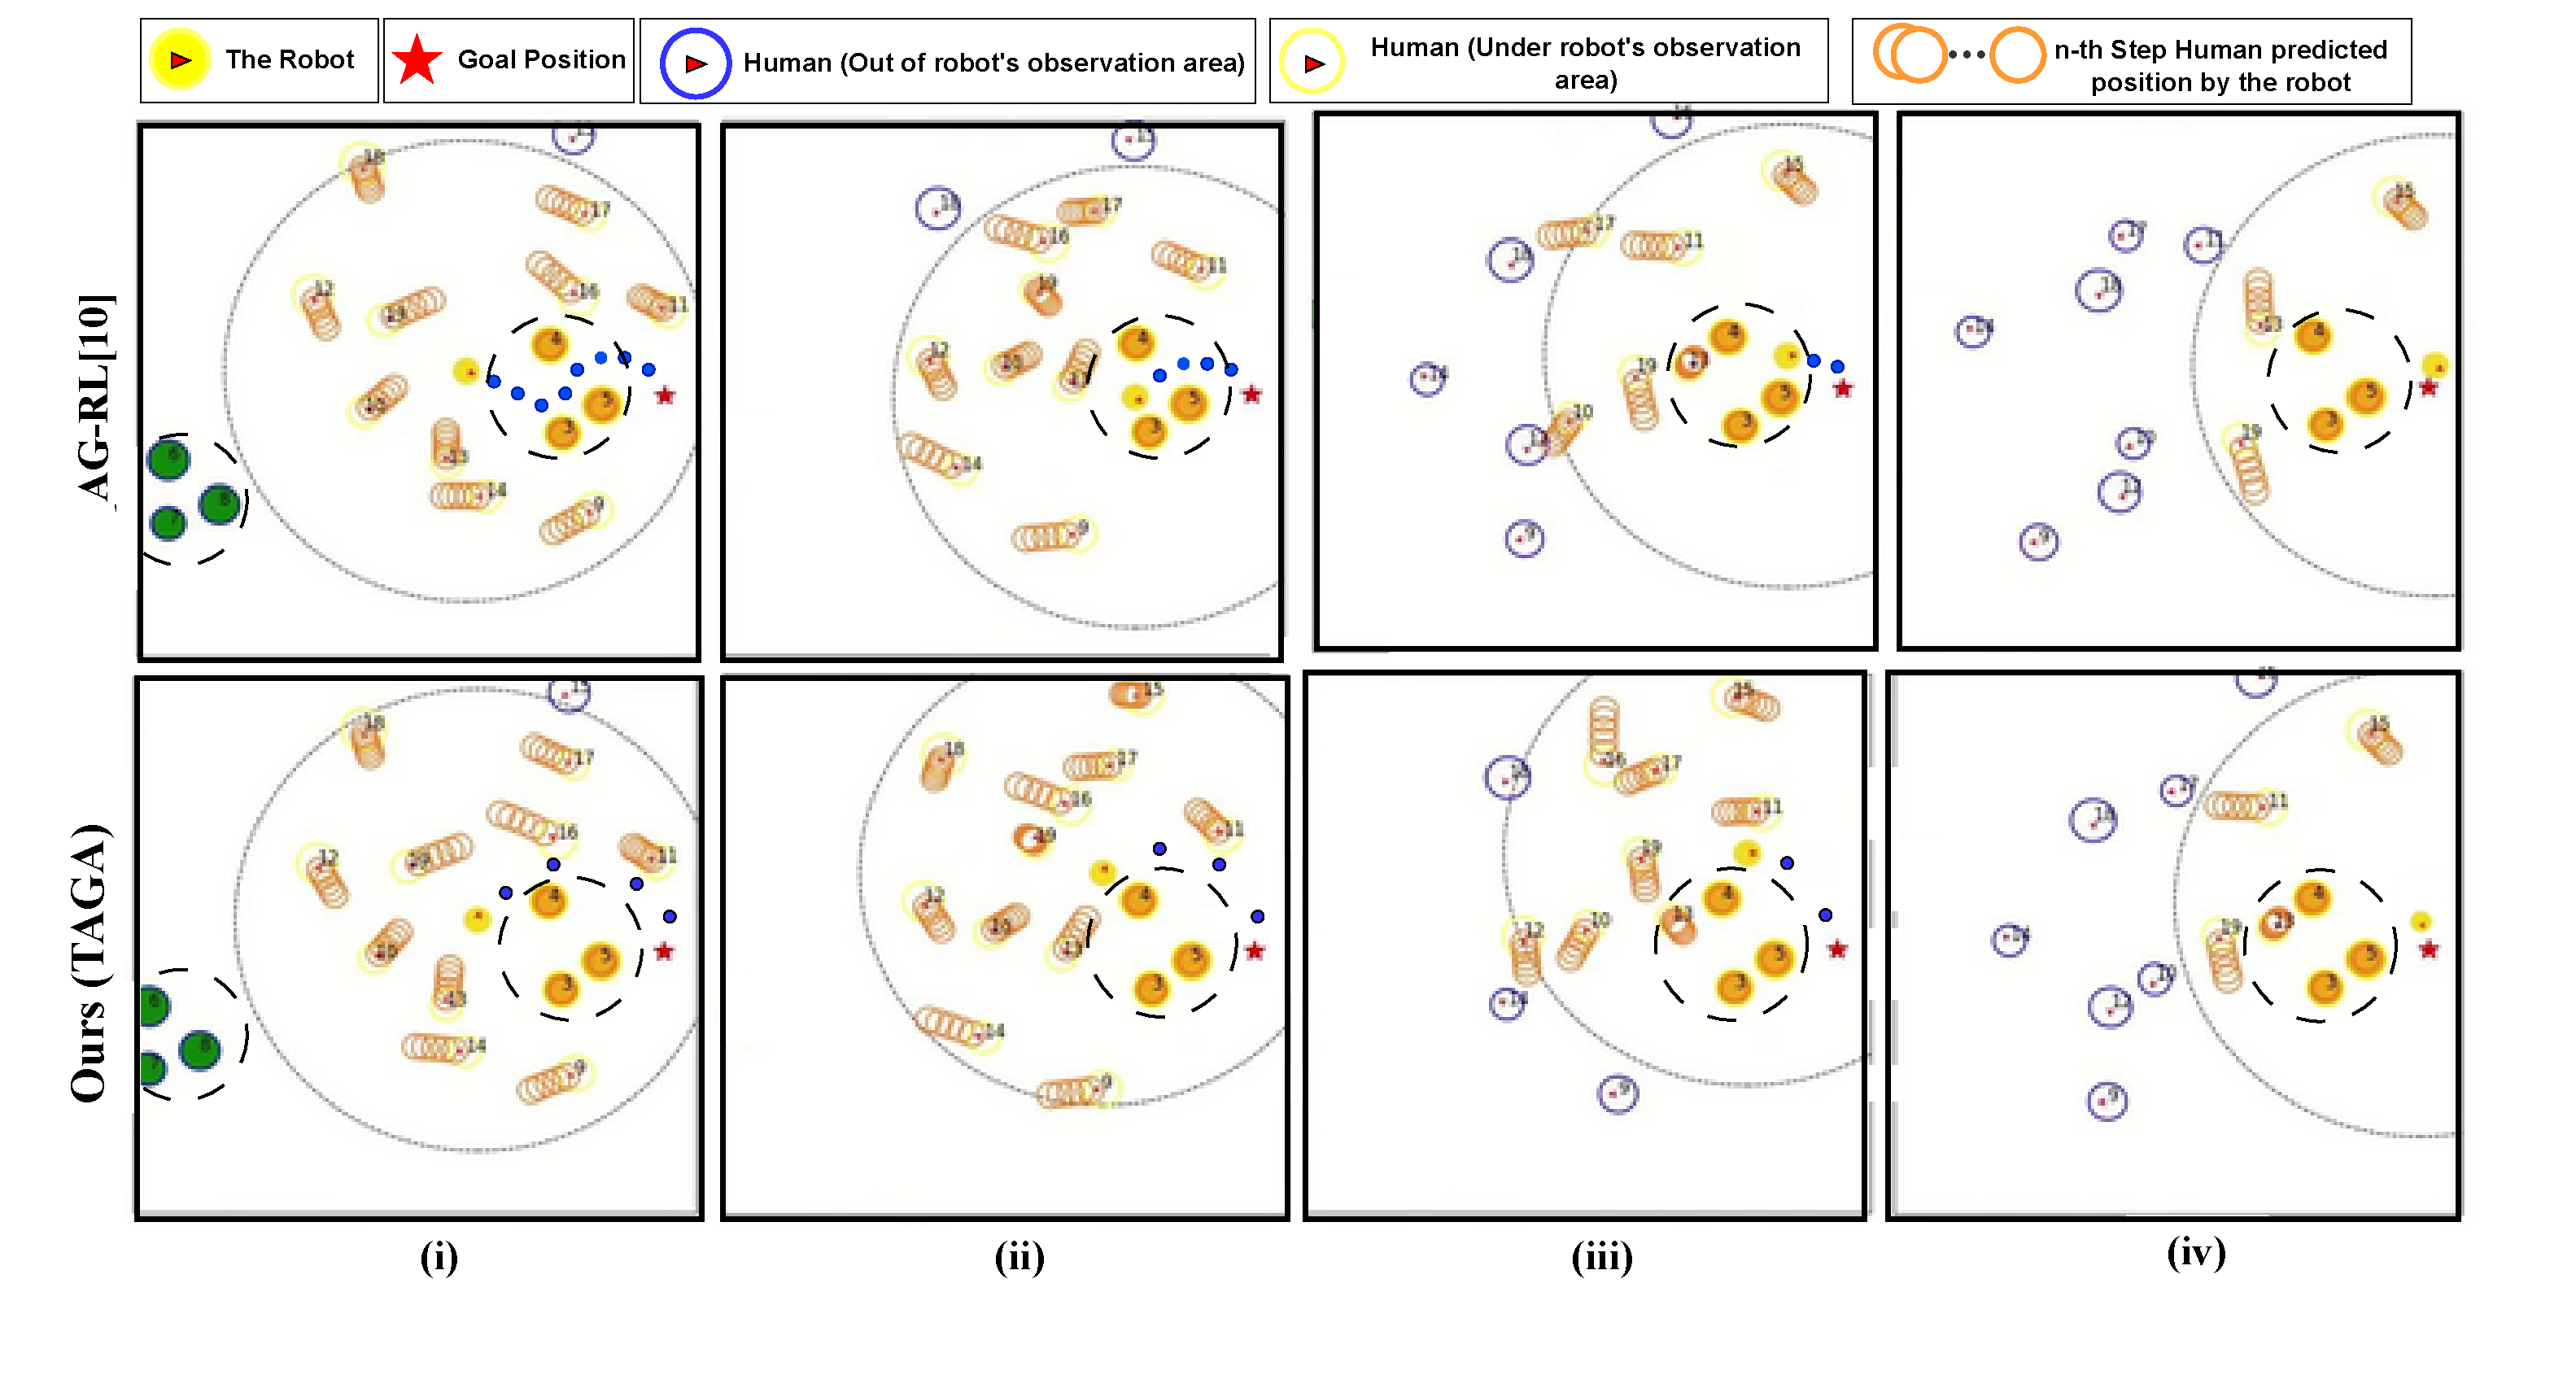
\includegraphics{figures/com.pdf}}
% %     \vspace{-25pt}
% %     \caption{\textbf{Comparison of our method (TAGA) and the state-of-the-art approach during the same testing episode, with identical randomized human and group placements.} The dotted circles represent group boundaries, while the small blue dots illustrate the robot's trajectory towards its goal. To ensure uninterrupted navigation, group collision constraints were disabled during the episode, allowing for continuous observation of the robot’s path planning and decision-making behavior.
% % }
% %     \vspace{-15pt}  
% %     \label{fig:sim-com}
% % \end{figure*}


% The integration of TAGA with an existing model $M$ follows a reactive approach based on group detection. \UT{The robot continuously monitors its surroundings and identifies human groups using spatial clustering, where group membership is determined by the proximity of individuals. Additionally, the robot calculates the average velocity of group members to identify cohesive movement patterns, further refining the group detection process.} If no group is detected, the robot follows the original navigation model $M(s)$, which provides actions for avoiding individual pedestrians. However, when a group is identified, the control switches to TAGA, which adjusts the robot’s trajectory using a tangent-based avoidance strategy. TAGA computes a path around the group boundary to ensure smooth and socially compliant navigation. Once the robot successfully passes the group, TAGA deactivates, and the control returns to $M(s)$, allowing the robot to resume its default navigation behavior.

% This modular design ensures that TAGA does not interfere with pre-trained policies when no groups are present, making it adaptable to any existing navigation model. The proposed approach effectively allows individual-based navigation frameworks to inherit group-awareness without retraining the entire model, thereby improving real-world applicability.

\section{EXPERIMENTAL SETUP}

\begin{figure*}[t]
    \centering
    \resizebox{\textwidth}{!}{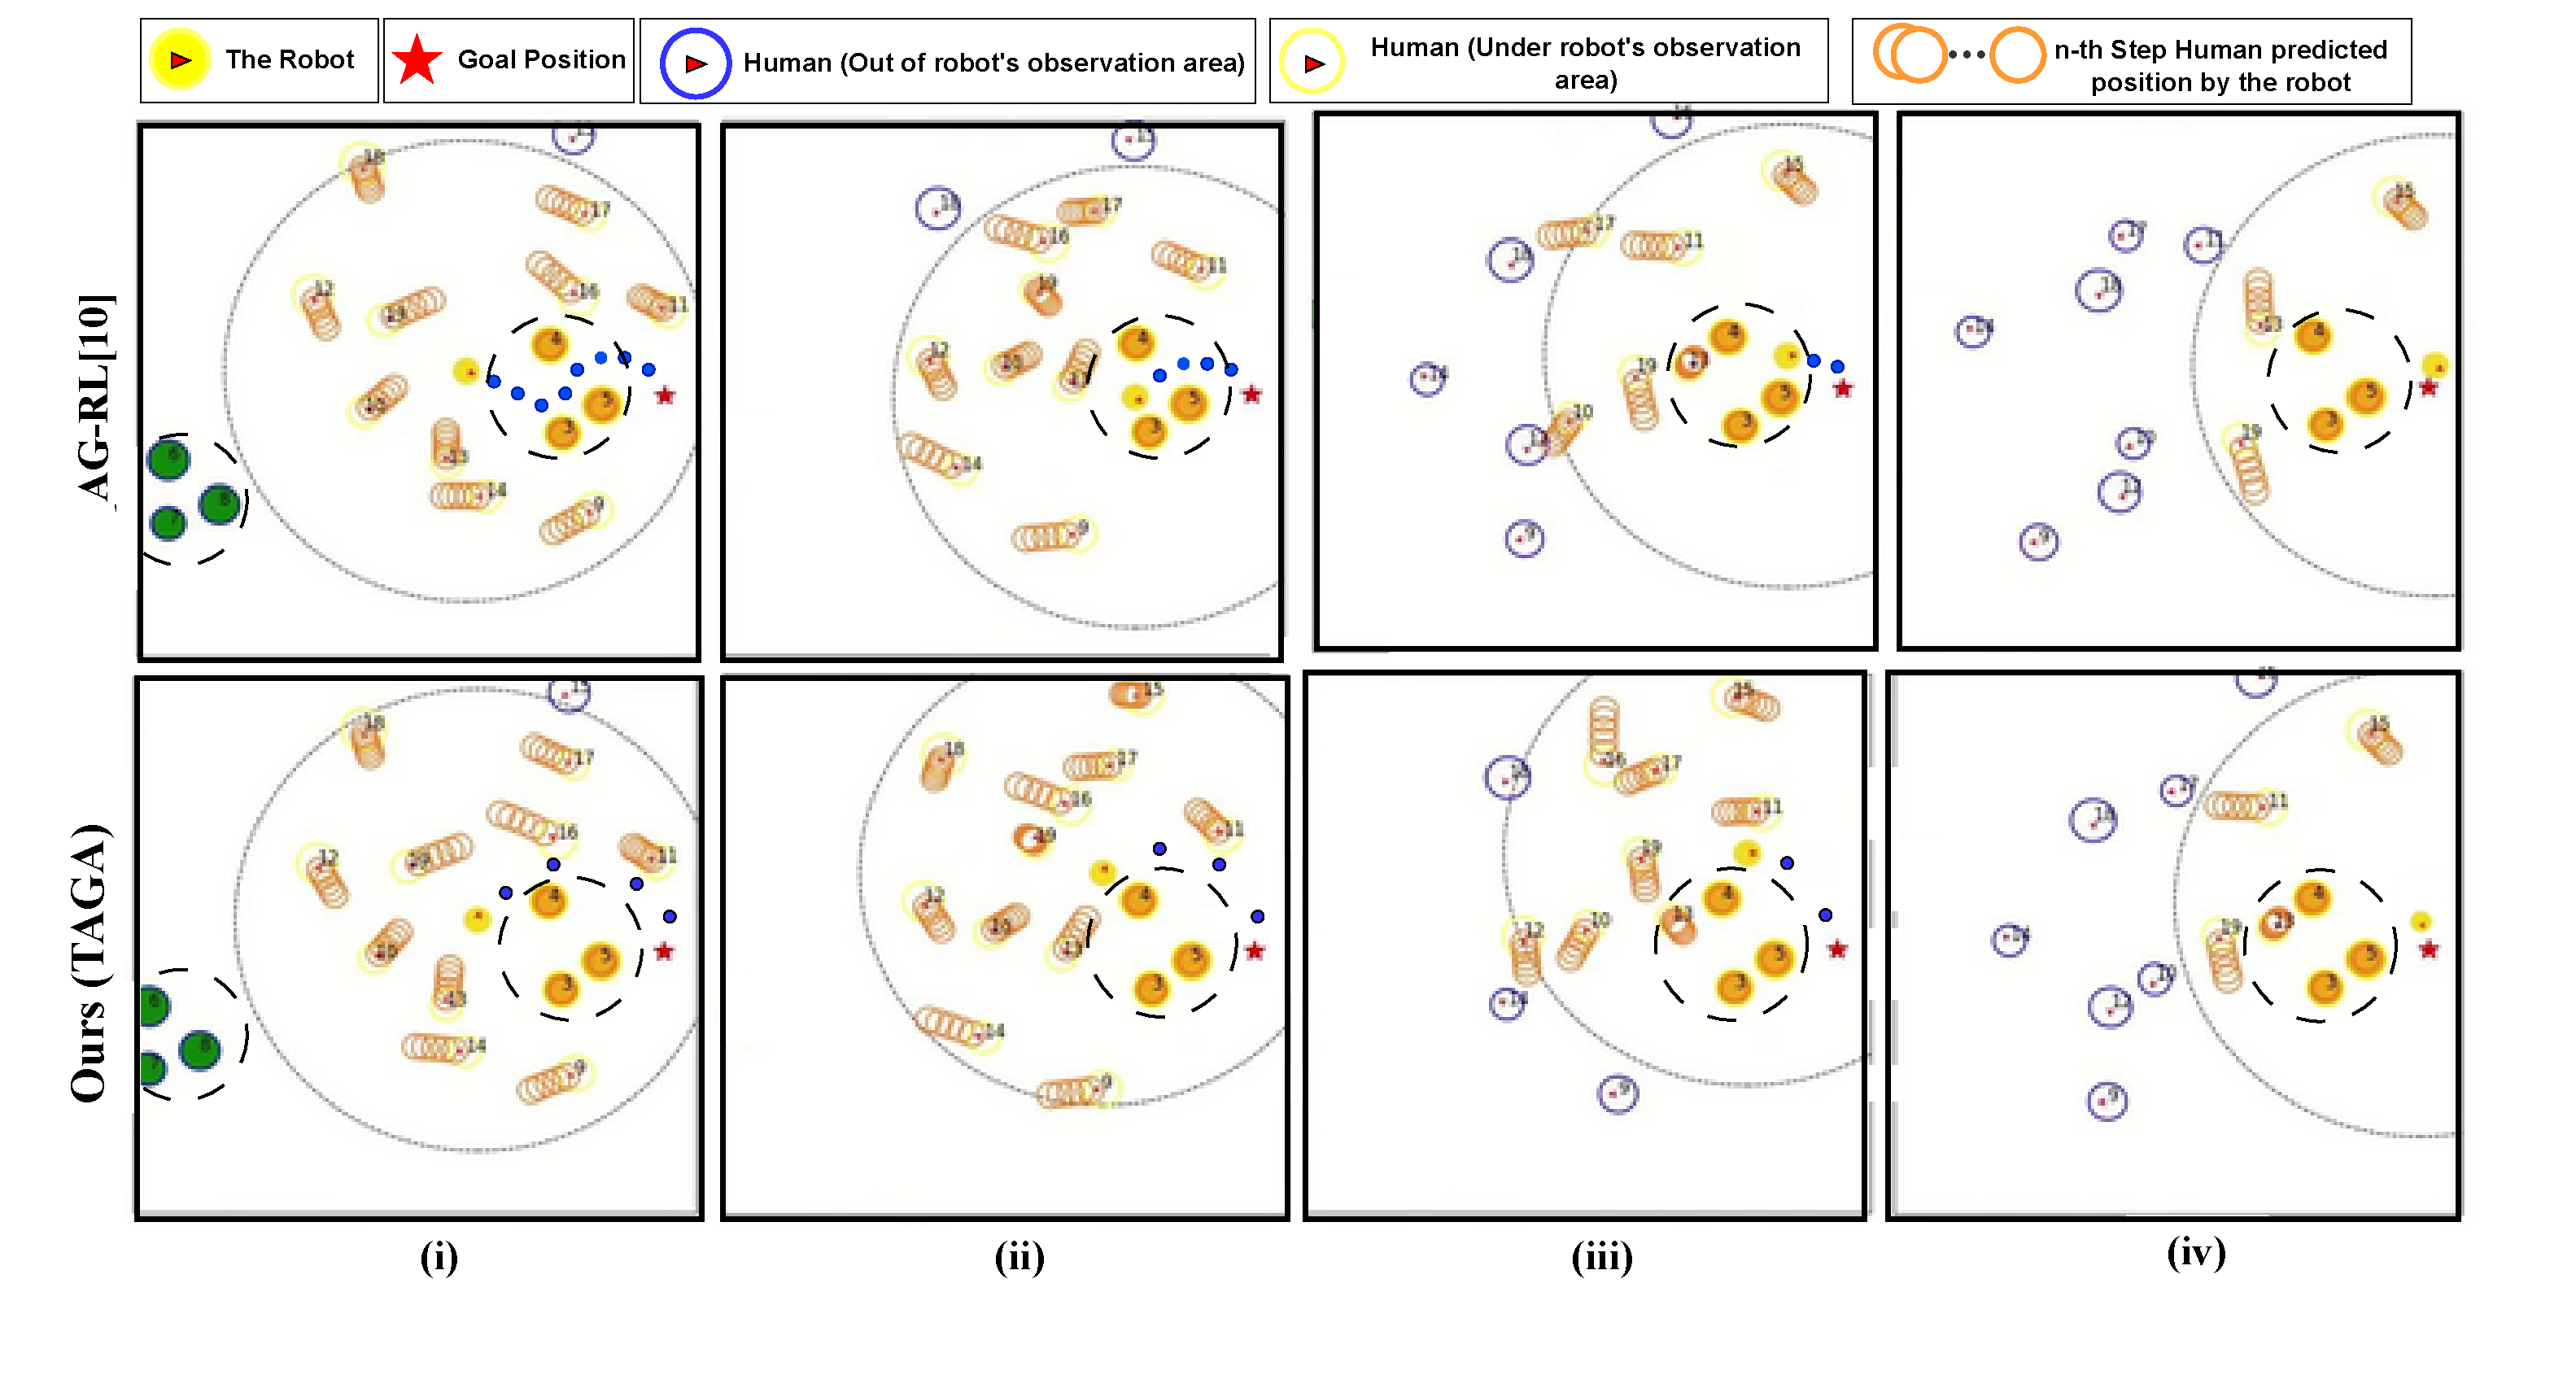
\includegraphics{figures/com.pdf}}
    \vspace{-25pt}
    \caption{\textbf{Comparison of our method (TAGA) and the state-of-the-art approach during the same testing episode, with identical randomized human and group placements.} The dotted circles represent group boundaries, while the small blue dots illustrate the robot's trajectory towards its goal. To ensure uninterrupted navigation, group collision constraints were disabled during the episode, allowing for continuous observation of the robot’s path planning and decision-making behavior.\UT{Try to address the 3rd review of reviwer 31289 and try to explain in qualilative sub section}
 }
    \vspace{-15pt}  
    \label{fig:sim-com}
\end{figure*}

\subsection{Simulation Environment}
We extend the crowd simulation framework from \cite{liu2023intention}, featuring a 12m × 12m space with up to 20 dynamic humans and a holonomic robot with 5m sensing range. Our key contribution is integrating realistic group behaviors alongside individual pedestrians. Groups are detected in real-time using DBSCAN clustering ($\epsilon = 1.5$m, minimum size = 2) rather than ground truth labels. \UT{addressing reviewer concerns about oversimplified detection.}

Dynamic groups follow leader-follower dynamics where a randomly selected leader navigates using ORCA while followers maintain cohesion through velocity adjustment: $v_i = v_{leader} + k(c - p_i)$, where $k$ is the cohesion factor and $c$ is the group centroid. Static groups remain stationary, representing conversational clusters.

\subsection{Evaluation Scenarios}
To ensure robust evaluation, we test across five diverse scenarios (100 episodes each):

\begin{itemize}
\item \textbf{Dense Groups} (20 episodes): 4 groups in 8m × 8m space, testing navigation through tight formations
\item \textbf{Mixed 50-50} (20 episodes): 8 individuals and 8 grouped humans, evaluating mixed crowd handling
\item \textbf{Dynamic Groups} (20 episodes): 3 moving groups with leader-follower dynamics
\item \textbf{Crossing Groups} (20 episodes): Groups traversing perpendicular to robot's path
\item \textbf{Groups Only} (20 episodes): All 18 humans in groups, no individuals
\end{itemize}

% This diverse set addresses the reviewer's requirement for "dense groups, mixed scenarios, and dynamic formations" while testing TAGA's adaptability.

\subsection{Metrics}
We evaluate using traditional navigation metrics and our proposed Group Collision Rate:

\textbf{Terminal States}: Success Rate (SR), Collision Rate (CR), and Timeout Rate (TR), where SR + CR + TR = 1.

% \textbf{Group Collision Rate (GCR)}: Measures the percentage of navigation time spent within group boundaries:
% \begin{equation}
% \text{GCR} = \frac{1}{T} \sum_{t=1}^{T} \mathbb{I}(d(r_t, c_j) < R_j) \times 100\%
% \end{equation}
% where $\mathbb{I}$ is the indicator function, $d(r_t, c_j)$ is robot distance to group $j$'s centroid, and $R_j$ is the group radius. Crucially, GCR operates independently of terminal states, providing continuous assessment throughout episodes.

\textbf{Group Collision Rate (GCR)}: Measures the percentage of navigation time during which the robot violates other groups' boundaries:
\begin{equation}
\text{GCR} = \frac{1}{T} \sum_{t=1}^{T} \mathbb{I}(d(r_t, c_j) < R_j) \times 100\%,
\end{equation}
where $T = t_{\text{episode}} \cdot f_{\text{ctrl}}$ is the total number of discrete control time steps, and the controller frequency is fixed at $f_{\text{ctrl}} = 10$~Hz throughout all experiments. $\mathbb{I}(\cdot)$ is the indicator function that returns $1$ if the robot is inside another group's region and $0$ otherwise, $d(r_t, c_j)$ denotes the Euclidean distance between the robot position at time step $t$ and group $j$'s centroid $c_j$, and $R_j$ is the group radius. Since GCR is evaluated at every control step, it provides a continuous assessment of group-aware behavior across the entire episode, independent of terminal success or failure. \UT{Try to address the 4th review of reviwer 31281}



\textbf{Efficiency}: Navigation Time (NT) and Path Length (PL) for successful episodes.

% \subsection{Implementation Details}
% We evaluate four baseline methods—ORCA \cite{orca}, Social Force \cite{helbing1995social}, DS-RNN \cite{liu2020decentralized}, and AG-RL \cite{liu2023intention} with and without TAGA integration. Key parameters include: safety margin $S = 0.5$m, critical distance $d_{critical} = 0.3$m, personal distance $d_{personal} = 0.5$m, and detection confidence threshold $\tau = 0.8$. All methods are tested on identical scenarios using fixed random seeds for reproducibility. The safety controller operates at 10Hz, ensuring real-time collision avoidance during group maneuvers.
\subsection{Implementation Details}
We evaluate four baseline methods—ORCA \cite{orca}, Social Force \cite{helbing1995social}, DS-RNN \cite{liu2020decentralized}, and AG-RL \cite{liu2023intention} with and without TAGA integration. Key parameters include: safety margin $S = 0.5$m, critical distance $d_{critical} = 0.3$m, personal distance $d_{personal} = 0.5$m. All methods are tested on identical scenarios using fixed random seeds for reproducibility. The safety controller operates at 10Hz, ensuring real-time collision avoidance during group maneuvers.

% \vspace{-4pt}
% \section{CROWD ROBOT NAVIGATION BENCHMARK}
% \vspace{-12pt}
% \begin{figure*}[t]
%     \centering
%     \resizebox{\textwidth}{!}{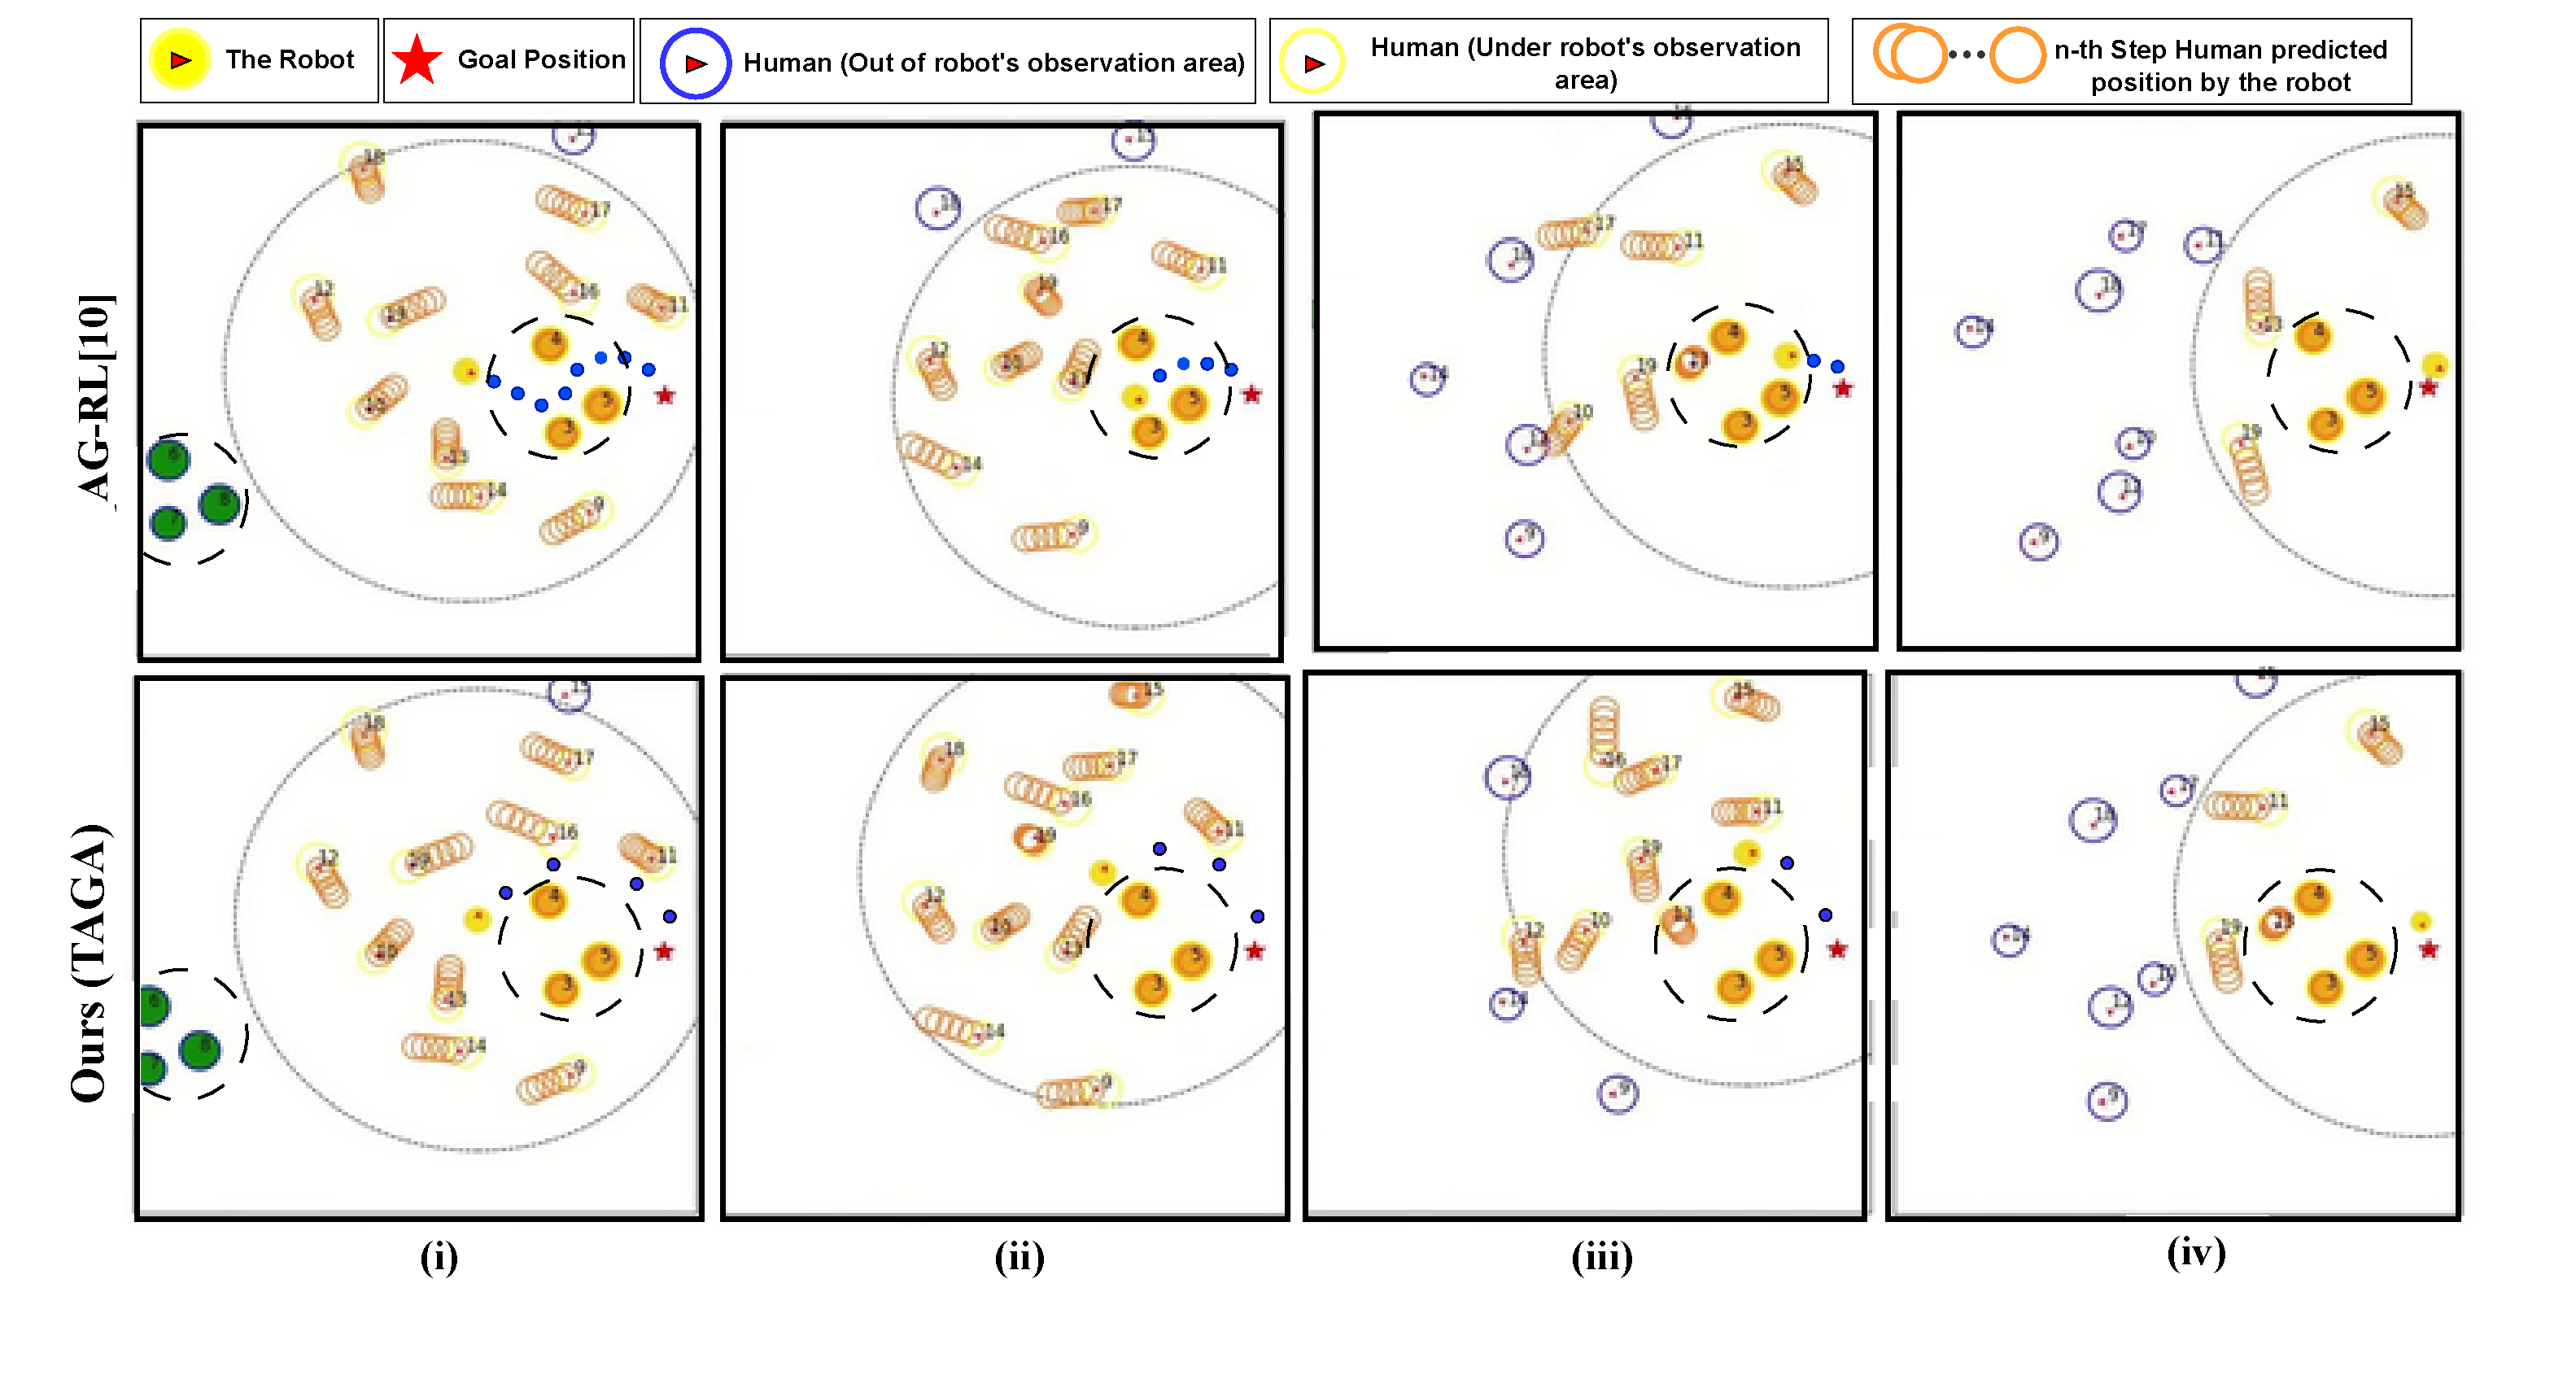
\includegraphics{figures/com.pdf}}
%     \vspace{-25pt}
%     \caption{\textbf{Comparison of our method (TAGA) and the state-of-the-art approach during the same testing episode, with identical randomized human and group placements.}  The dotted circles represent group boundaries, while the small blue dots illustrate the robot's trajectory towards its goal. To ensure uninterrupted navigation, group collision constraints were disabled during the episode, allowing for continuous observation of the robot’s path planning and decision-making behavior.
% }
%     \vspace{-15pt}  
%     \label{fig:sim-com}
% \end{figure*}

% \vspace{-2pt}
% \subsection{Simulation Environment}
% We build upon the simulation environment proposed in \cite{liu2023intention}, where a robot navigates through a dense 12m × 12m crowd space with up to 20 dynamic humans. The environment features a holonomic robot with a limited 5m sensor range and realistic human flow dynamics, ensuring continuous crowd interaction. Humans are controlled by the ORCA algorithm, reacting only to other humans while remaining unaware of the robot's presence.

% In contrast to \cite{liu2023intention}, we extend this environment by introducing human group behaviors alongside individual pedestrians. As shown in Fig. \ref{fig:sim-com}, groups are visually represented by similar-colored circles, indicating pedestrians that move together or standing close to each other. 
% This modification enables a more realistic evaluation of group-aware navigation strategies while preserving the original framework's crowd dynamics.
% \vspace{-10pt}
% \subsection{Human Group Simulation}
% We model human groups using a spatial representation, where each group is defined by a centroid $c$ and a radius $r$. The centroid $c$ is computed as the average position of all group members, where $N$ represents the total number of members in the group, and $p_i = (x_i, y_i)$ denotes the position of the $i$-th group member. Each group member is positioned within a maximum allowable distance $r$ from the centroid, ensuring spatial cohesion within the group. The set of all group members is represented by $G$:

% \begin{equation}
% c = \frac{1}{N} \sum_{i=1}^{N} p_i, \quad \| p_i - c \| \leq r, \quad \forall i \in G
% \end{equation}

% For dynamic groups, a leader is selected randomly from the group members:  

% \begin{equation}
% \text{leader} = \text{random}(G)
% \end{equation}

% We model human groups spatially, where each group is defined by a centroid $c$ and radius $r$. The centroid is the average position of all members, with $p_i = (x_i, y_i)$ representing the position of the $i$-th member. The members are constrained within a maximum distance $r$ from the centroid, ensuring spatial cohesion. The set of all members is denoted by $G$, and the spatial constraints are expressed as $c = \frac{1}{N} \sum_{i=1}^{N} p_i$, where $\quad \| p_i - c \| \leq r$ and $\quad \forall i \in G$.

% For dynamic groups, a leader is randomly selected as $\text{leader} = \text{random}(G)$.


% The leader follows ORCA-based navigation\cite{orca}, where $p_{\text{leader}}(t)$ represents the leader's position at time $t$, $v_{\text{orca}}$ is the velocity computed using the ORCA algorithm, and $\Delta t$ is the simulation time step:

% $$
% p_{\text{leader}}(t+1) = p_{\text{leader}}(t) + v_{\text{orca}} \cdot \Delta t \eqno{(3)}
% $$
% \vspace{-12pt} % Reduce space before

% \begin{equation}
% p_{\text{leader}}(t+1) = p_{\text{leader}}(t) + v_{\text{orca}} \cdot \Delta t
% \end{equation}
% \vspace{-14pt} % Reduce space before


% Each follower in the group maintains cohesion by adjusting its velocity relative to the leader and the group centroid. Here, $v_i$ denotes the velocity of the $i$-th follower, $v_{\text{leader}}$ represents the velocity of the leader, and $k$ is a cohesion factor ensuring that members remain within the group:

% $$
% v_i = v_{\text{leader}} + k (c - p_i) \eqno{(4)}
% $$
% \vspace{-10pt} % Reduce space before
% \begin{equation}
% v_i = v_{\text{leader}} + k (c - p_i)
% \end{equation}
% \vspace{-15pt} % Reduce space before

% For static groups, all members remain stationary, with $G_{\text{static}}$ representing the set of static group members, where $v_i = 0$ for all $i \in G_{\text{static}}$.

% This formulation ensures a structured simulation of both dynamic and static groups, allowing robots to interact with more realistic crowd behaviors in navigation environments.
% \vspace{-2pt}
% \subsection{Task}
% The robot, represented by a yellow circle with an arrow inside (Fig. \ref{fig:sim-com}), starts at one side of the environment, typically opposite to the goal, which is marked as a star in Fig. \ref{fig:sim-com}. The primary objective of the robot is to navigate toward the goal while avoiding collisions with individual humans, group members, and group boundaries. To prevent indefinite simulations in cases where a valid navigation path is not found, we impose a time limit of 197 steps. The robot navigates freely within the environment as the surrounding crowd, consisting of both individual pedestrians and group members, moves dynamically and unpredictably. However, humans in the crowd can traverse through group members without restrictions.

% \begin{figure}[!ht]
%     \centering
%     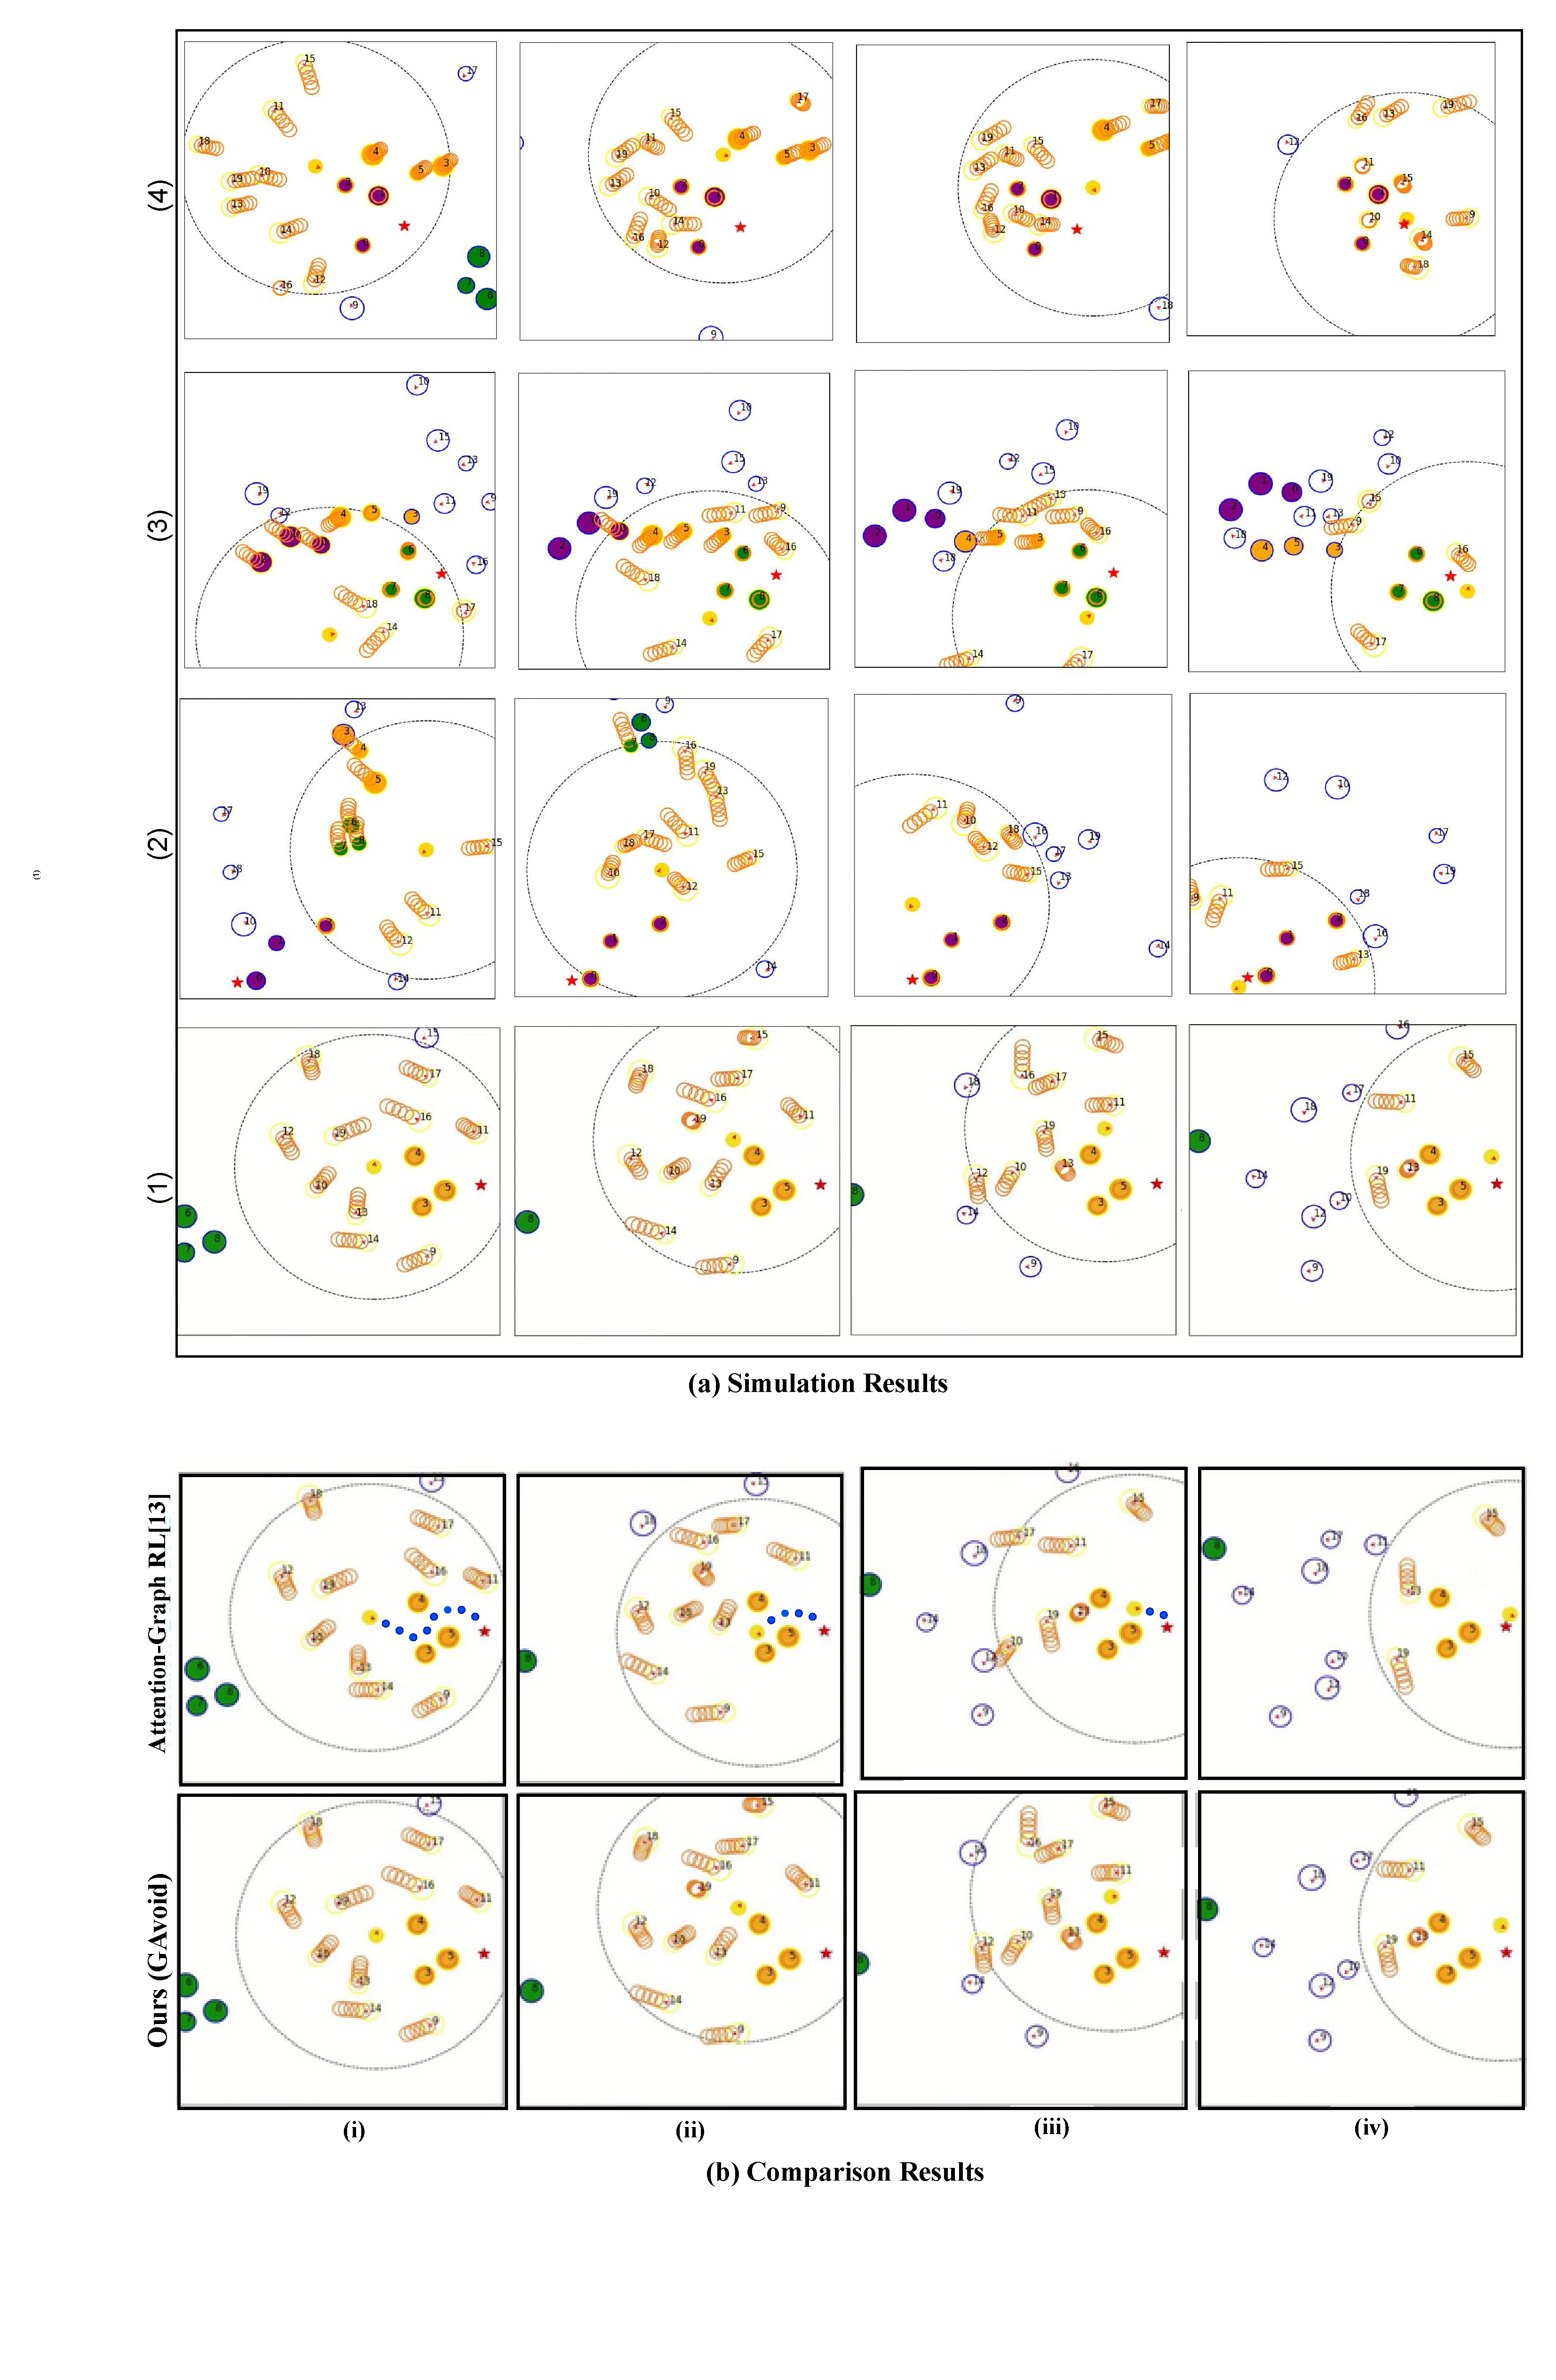
\includegraphics[width=0.5\textwidth]{figures/res.pdf}
%     \caption{Simulations Steps of different Configuration of Environments}
%     \label{fig:sim-res-1}
% \end{figure}
% \begin{figure}
%       \centering
%       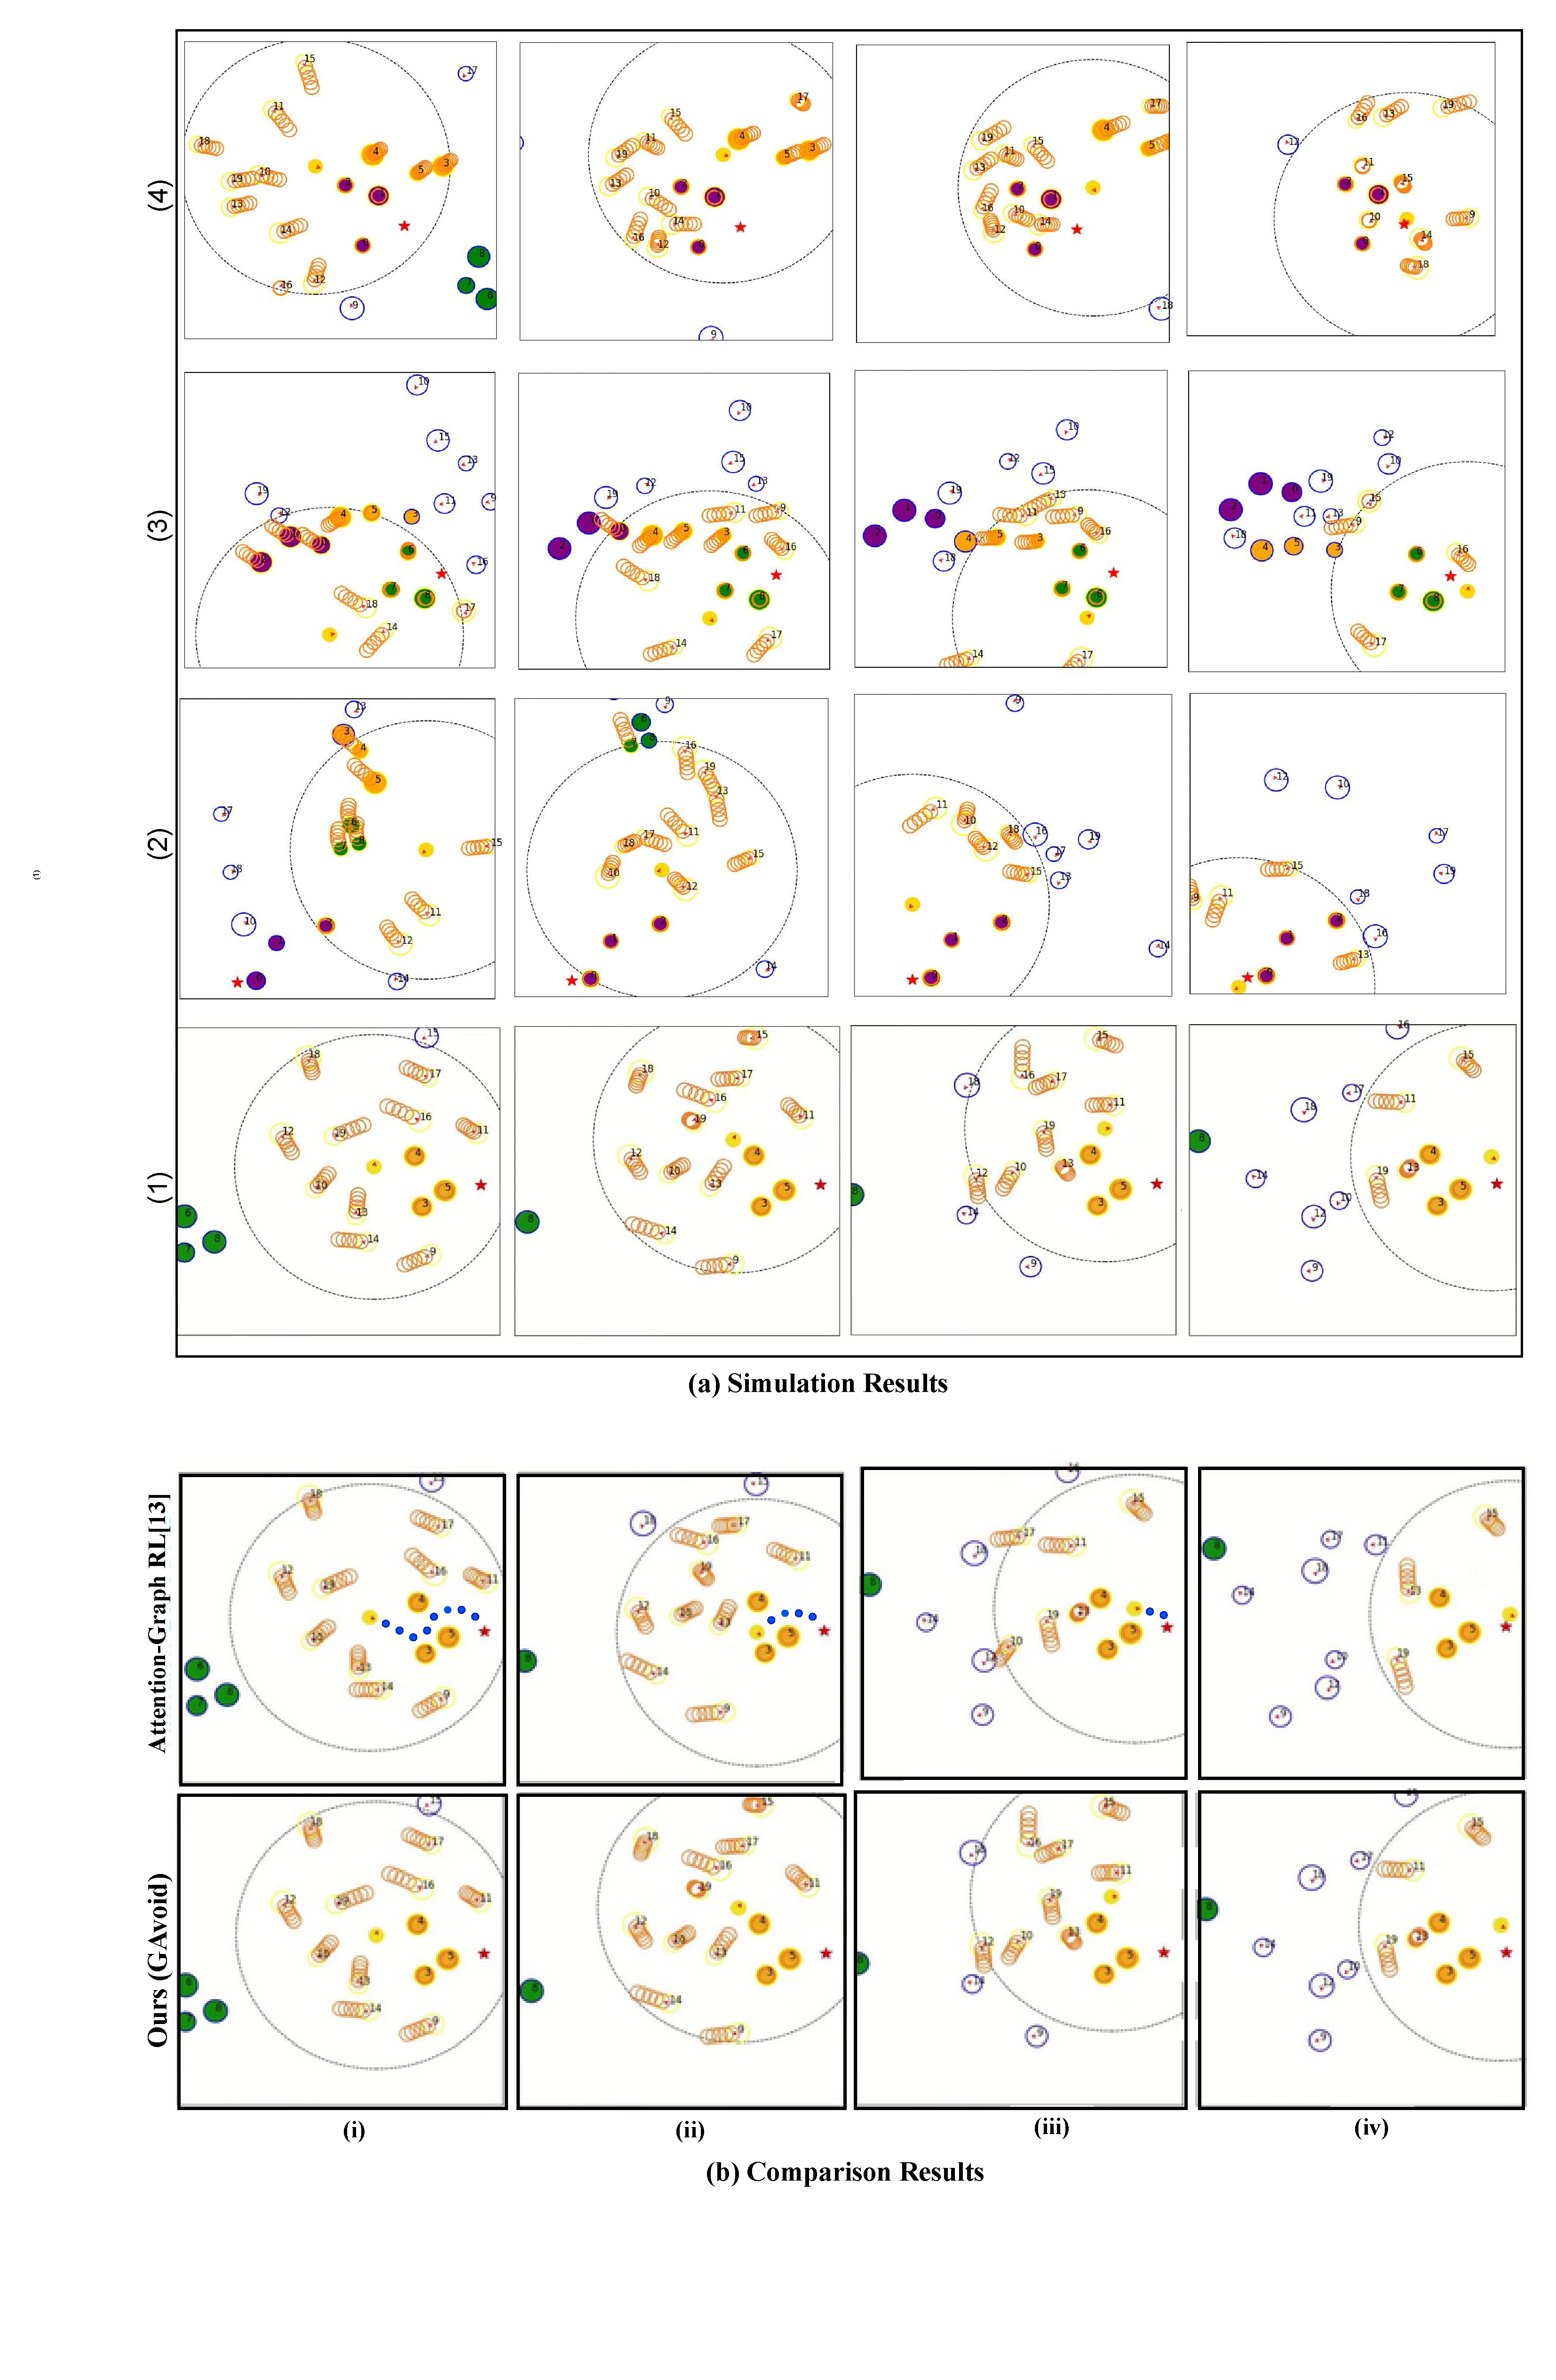
\includegraphics[scale=0.7]{figures/res.pdf}
%       \caption{Comparison with other models}
%       \label{fig:sim-com-1}
%    \end{figure}

% \vspace{-5pt}
% \vspace{-5pt} 
% \subsection{Benchmark Setup}
% To evaluate the impact of human groups on robot navigation, we conduct the benchmark in two experimental phases. First, we evaluate the performance of four widely used navigation frameworks—ORCA \cite{orca}, Social Force \cite{helbing1995social}, DS-RNN \cite{liu2020decentralized}, and AG-RL \cite{liu2023intention} to analyze their ability to navigate in the presence of individual humans and human groups. Next, we integrate our proposed TAGA mechanism into these models to examine how well they adapt to group-aware navigation. For instance, ORCA + TAGA allows ORCA to incorporate reactive group avoidance, ensuring that it respects group boundaries. Similar integration is applied to the other methods to assess their performance with group-awareness.

% Each approach is tested under identical conditions to ensure a fair comparison. The experiments are conducted across different configurations, adjusting crowd density, group sizes, and movement dynamics to assess performance across various scenarios.

% Furthermore, to quantify the effectiveness of group-aware navigation, GCR serves as a key performance metric, alongside traditional evaluation criteria such as SR, CR, and navigation efficiency. This benchmark setup provides a structured and reproducible evaluation of navigation models in realistic human environments.

% To ensure reliable evaluation, all methods are tested on 100 randomly generated unseen cases. If a collision occurs during an episode, the simulation is immediately terminated to reflect real-world navigation constraints. Consequently, the total of all failure rates, including Collision Rate (CR), Timeout Rate (TR), and GCR, along with the SR, always equals 1, expressed as $CR + TR + GCR + SR = 1$. Note that all time measurements are in seconds, and all distance measurements are in meters.
% \vspace{-5pt} 
% \subsection{Metrics}
% Our evaluation focuses on four key aspects: (1) robot navigation performance, (2) safety considerations, (3) real-time performance, and (4) group-aware navigation.

% \textbf{Real-Time Performance:} This metric evaluates the overall success of the navigation attempts, including the Success Rate (SR), which is the percentage of trials where the robot successfully reached the goal without colliding or exceeding the time limit.

% \textbf{Robot Navigation Performance:} These metrics assess the robot’s efficiency in reaching the goal while optimizing movement. This includes Navigation Time (NT), the average time required for the robot to reach the goal across all trials, and Path Length (PL), the total distance traveled by the robot from start to goal, averaged over all trials.

% \textbf{Safety Considerations:} These metrics quantify the safety of the robot’s navigation by measuring collision risks. They include CR, the number of trials where the robot collided with a human or group boundary, and TR, the percentage of trials where the robot failed to reach the goal within the allotted time.

% \textbf{Real-Time Performance:} This metric evaluates the overall success of the navigation attempts.

% \begin{itemize}
%     \item Success Rate (SR): The percentage of trials where the robot successfully reached the goal without colliding or exceeding the time limit.  
% \end{itemize}

% \textbf{Robot Navigation Performance:} These metrics assess the robot’s efficiency in reaching the goal while optimizing movement.

% \begin{itemize}
%     \item Navigation Time (NT): The average time required for the robot to reach the goal across all trials.  
%     \item Path Length (PL): The total distance traveled by the robot from start to goal, averaged over all trials.  
% \end{itemize}

% \textbf{Safety Considerations:} These metrics quantify the safety of the robot’s navigation by measuring collision risks.

% \begin{itemize}
%     \item Collision Rate (CR): The number of trials where the robot collided with a human or group boundary.  
%     \item Timeout Rate (TR): The percentage of trials where the robot failed to reach the goal within the allotted time.  
% \end{itemize}

% \textbf{Group-Aware Navigation:} To quantify the effectiveness of group-aware navigation, GCR measures how well the robot avoids intruding into human groups. Here, GCR is defined as the proportion of time the robot remains within a group’s spatial boundary during navigation:

% % $$
% % GCR = \frac{\sum_{t=1}^{T} \mathbb{I} (p_r(t) \in G)}{T} \eqno{(6)}
% % $$
% \vspace{-10pt}
% \begin{equation}
% GCR = \frac{\sum_{t=1}^{T} \mathbb{I} (p_r(t) \in G)}{T}
% \end{equation}
% \vspace{-15pt}

% where, $T$ is the total number of time steps in a trial, $p_r(t)$ represents the position of the robot at time step $t$, $\mathbb{I} (p_r(t) \in G)$ is an indicator function that returns 1 if the robot is inside a group's spatial boundary and 0 otherwise.


% We test all methods with 500 random unseen test cases. Our metrics include navigation metrics and social metrics. The navigation metrics measure the quality of the navigation and include the percentage success rate (SR), average navigation time (NT) in seconds, and path length (PL) in meters of the successful episodes. 



% \begin{figure}[t]
%       \centering
%       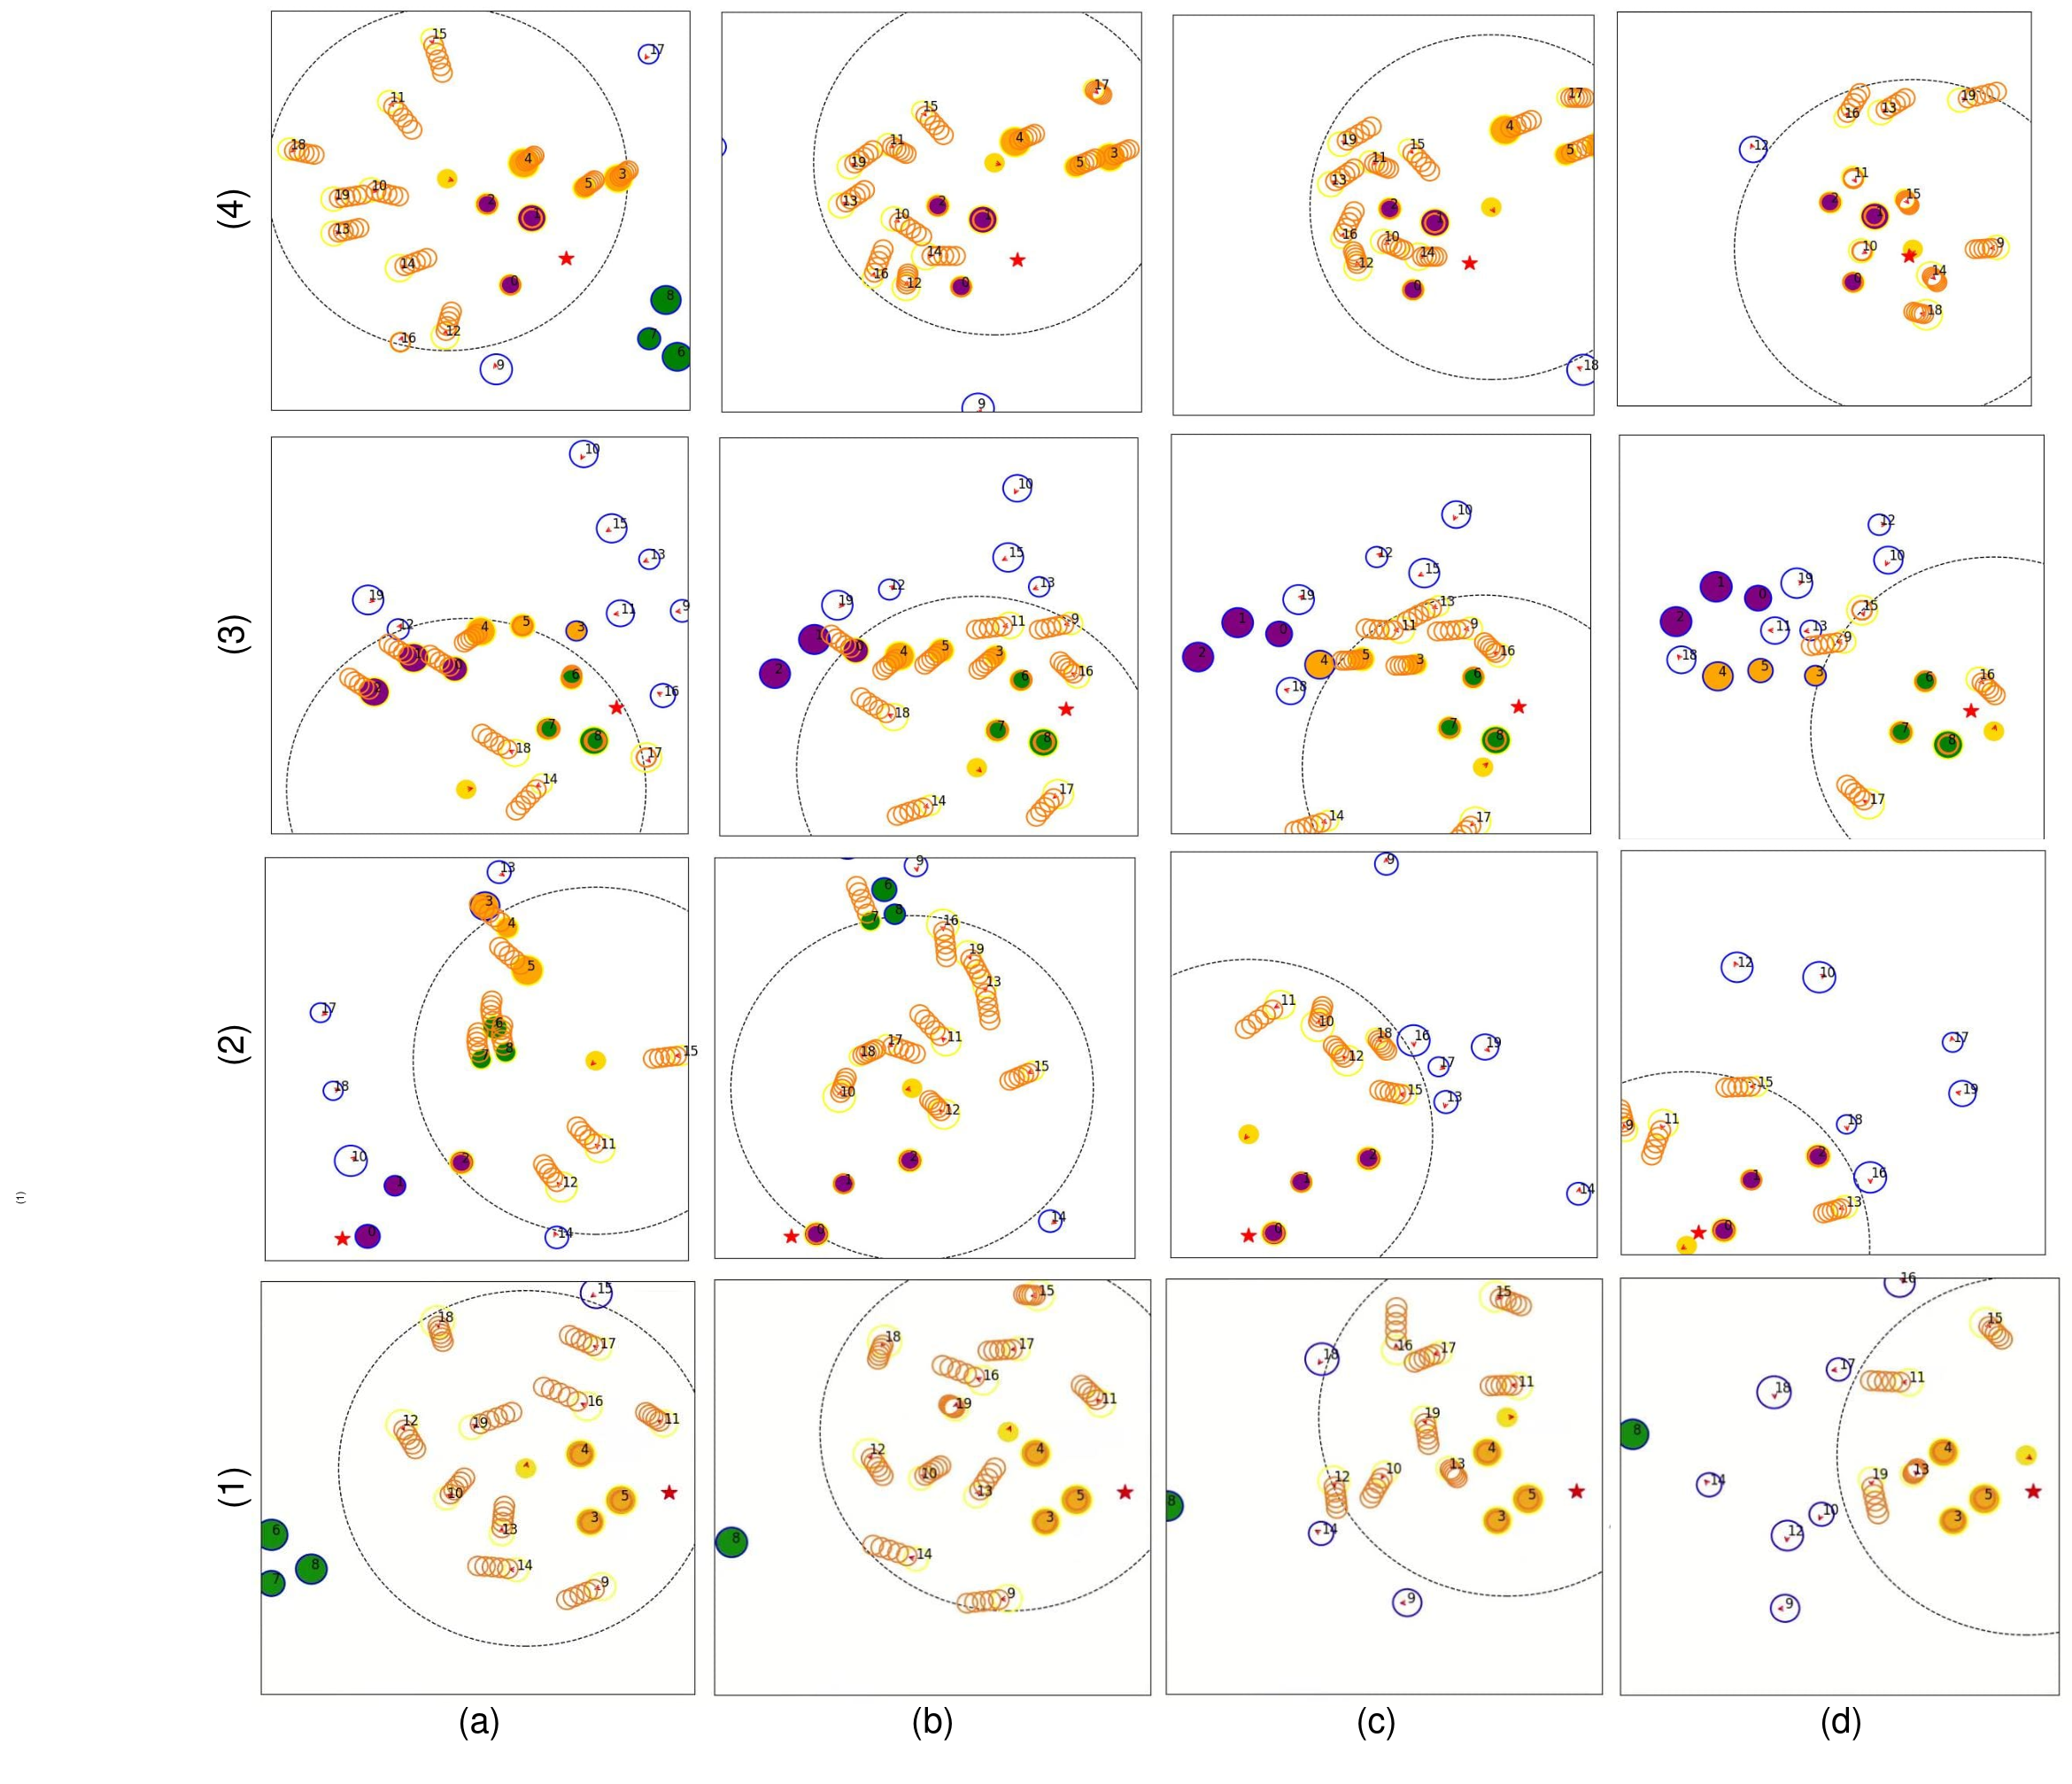
\includegraphics[scale=0.4]{figures/res-sim.png}
%       \caption{Simulations Steps of different Configuration of Environments}
%       \label{fig:sim-res-1}
%    \end{figure}























% \section{MATH}

% Before you begin to format your paper, first write and save the content as a separate text file. Keep your text and graphic files separate until after the text has been formatted and styled. Do not use hard tabs, and limit use of hard returns to only one return at the end of a paragraph. Do not add any kind of pagination anywhere in the paper. Do not number text heads-the template will do that for you.

% Finally, complete content and organizational editing before formatting. Please take note of the following items when proofreading spelling and grammar:

% \subsection{Abbreviations and Acronyms} Define abbreviations and acronyms the first time they are used in the text, even after they have been defined in the abstract. Abbreviations such as IEEE, SI, MKS, CGS, sc, dc, and rms do not have to be defined. Do not use abbreviations in the title or heads unless they are unavoidable.

% \subsection{Units}

% \begin{itemize}

% \item Use either SI (MKS) or CGS as primary units. (SI units are encouraged.) English units may be used as secondary units (in parentheses). An exception would be the use of English units as identifiers in trade, such as Ò3.5-inch disk driveÓ.
% \item Avoid combining SI and CGS units, such as current in amperes and magnetic field in oersteds. This often leads to confusion because equations do not balance dimensionally. If you must use mixed units, clearly state the units for each quantity that you use in an equation.
% \item Do not mix complete spellings and abbreviations of units: ÒWb/m2Ó or Òwebers per square meterÓ, not Òwebers/m2Ó.  Spell out units when they appear in text: Ò. . . a few henriesÓ, not Ò. . . a few HÓ.
% \item Use a zero before decimal points: Ò0.25Ó, not Ò.25Ó. Use Òcm3Ó, not ÒccÓ. (bullet list)

% \end{itemize}


% \subsection{Equations}

% The equations are an exception to the prescribed specifications of this template. You will need to determine whether or not your equation should be typed using either the Times New Roman or the Symbol font (please no other font). To create multileveled equations, it may be necessary to treat the equation as a graphic and insert it into the text after your paper is styled. Number equations consecutively. Equation numbers, within parentheses, are to position flush right, as in (1), using a right tab stop. To make your equations more compact, you may use the solidus ( / ), the exp function, or appropriate exponents. Italicize Roman symbols for quantities and variables, but not Greek symbols. Use a long dash rather than a hyphen for a minus sign. Punctuate equations with commas or periods when they are part of a sentence, as in

% $$
% \alpha + \beta = \chi \eqno{(1)}
% $$

% Note that the equation is centered using a center tab stop. Be sure that the symbols in your equation have been defined before or immediately following the equation. Use Ò(1)Ó, not ÒEq. (1)Ó or Òequation (1)Ó, except at the beginning of a sentence: ÒEquation (1) is . . .Ó

% \subsection{Some Common Mistakes}
% \begin{itemize}


% \item The word ÒdataÓ is plural, not singular.
% \item The subscript for the permeability of vacuum ?0, and other common scientific constants, is zero with subscript formatting, not a lowercase letter ÒoÓ.
% \item In American English, commas, semi-/colons, periods, question and exclamation marks are located within quotation marks only when a complete thought or name is cited, such as a title or full quotation. When quotation marks are used, instead of a bold or italic typeface, to highlight a word or phrase, punctuation should appear outside of the quotation marks. A parenthetical phrase or statement at the end of a sentence is punctuated outside of the closing parenthesis (like this). (A parenthetical sentence is punctuated within the parentheses.)
% \item A graph within a graph is an ÒinsetÓ, not an ÒinsertÓ. The word alternatively is preferred to the word ÒalternatelyÓ (unless you really mean something that alternates).
% \item Do not use the word ÒessentiallyÓ to mean ÒapproximatelyÓ or ÒeffectivelyÓ.
% \item In your paper title, if the words Òthat usesÓ can accurately replace the word ÒusingÓ, capitalize the ÒuÓ; if not, keep using lower-cased.
% \item Be aware of the different meanings of the homophones ÒaffectÓ and ÒeffectÓ, ÒcomplementÓ and ÒcomplimentÓ, ÒdiscreetÓ and ÒdiscreteÓ, ÒprincipalÓ and ÒprincipleÓ.
% \item Do not confuse ÒimplyÓ and ÒinferÓ.
% \item The prefix ÒnonÓ is not a word; it should be joined to the word it modifies, usually without a hyphen.
% \item There is no period after the ÒetÓ in the Latin abbreviation Òet al.Ó.
% \item The abbreviation Òi.e.Ó means Òthat isÓ, and the abbreviation Òe.g.Ó means Òfor exampleÓ.

% \end{itemize}

% % ########################
% % ########################
% % ########################
% \section{USING THE TEMPLATE}

% Use this sample document as your LaTeX source file to create your document. Save this file as {\bf root.tex}. You have to make sure to use the cls file that came with this distribution. If you use a different style file, you cannot expect to get required margins. Note also that when you are creating your out PDF file, the source file is only part of the equation. {\it Your \TeX\ $\rightarrow$ PDF filter determines the output file size. Even if you make all the specifications to output a letter file in the source - if your filter is set to produce A4, you will only get A4 output. }

% It is impossible to account for all possible situation, one would encounter using \TeX. If you are using multiple \TeX\ files you must make sure that the ``MAIN`` source file is called root.tex - this is particularly important if your conference is using PaperPlaza's built in \TeX\ to PDF conversion tool.

% \subsection{Headings, etc}

% Text heads organize the topics on a relational, hierarchical basis. For example, the paper title is the primary text head because all subsequent material relates and elaborates on this one topic. If there are two or more sub-topics, the next level head (uppercase Roman numerals) should be used and, conversely, if there are not at least two sub-topics, then no subheads should be introduced. Styles named ÒHeading 1Ó, ÒHeading 2Ó, ÒHeading 3Ó, and ÒHeading 4Ó are prescribed.

% \subsection{Figures and Tables}

% Positioning Figures and Tables: Place figures and tables at the top and bottom of columns. Avoid placing them in the middle of columns. Large figures and tables may span across both columns. Figure captions should be below the figures; table heads should appear above the tables. Insert figures and tables after they are cited in the text. Use the abbreviation ÒFig. 1Ó, even at the beginning of a sentence.

% \begin{table}[!t]
% \caption{An Example of a Table}
% \label{table_example}
% \begin{center}
% \begin{tabular}{|c||c|}
% \hline
% One & Two\\
% \hline
% Three & Four\\
% \hline
% \end{tabular}
% \end{center}
% \end{table}


%    \begin{figure}[thpb]
%       \centering
%       \framebox{\parbox{3in}{We suggest that you use a text box to insert a graphic (which is ideally a 300 dpi TIFF or EPS file, with all fonts embedded) because, in an document, this method is somewhat more stable than directly inserting a picture.
% }}
%       %\includegraphics[scale=1.0]{figurefile}
%       \caption{Inductance of oscillation winding on amorphous
%        magnetic core versus DC bias magnetic field}
%       \label{figurelabel}
%    \end{figure}
   

% Figure Labels: Use 8 point Times New Roman for Figure labels. Use words rather than symbols or abbreviations when writing Figure axis labels to avoid confusing the reader. As an example, write the quantity ÒMagnetizationÓ, or ÒMagnetization, MÓ, not just ÒMÓ. If including units in the label, present them within parentheses. Do not label axes only with units. In the example, write ÒMagnetization (A/m)Ó or ÒMagnetization {A[m(1)]}Ó, not just ÒA/mÓ. Do not label axes with a ratio of quantities and units. For example, write ÒTemperature (K)Ó, not ÒTemperature/K.Ó

% \section{RESULTS AND ANALYSIS}

\subsection{Overall Performance Comparison}

\begin{table}[t]
\caption{Performance comparison with and without TAGA (500 episodes)}
\label{table:main-results}
\centering
\begin{tabular}{lcccccc}
\hline
\textbf{Method} & \textbf{SR↑} & \textbf{CR↓} & \textbf{TR↓} & \textbf{GCR↓} & \textbf{NT(s)} & \textbf{PL(m)} \\
\hline
AG-RL & 0.78 & 0.20 & 0.02 & 10.54\% & 15.47 & 21.54 \\
AG-RL+TAGA & \textbf{0.82} & \textbf{0.16} & \textbf{0.02} & 8.82\% & 16.79 & 22.68 \\
\hline
DS-RNN & 0.64 & 0.32 & 0.04 & 9.87\% & 17.23 & 22.15 \\
DS-RNN+TAGA & 0.66 & 0.29 & 0.05 & 4.13\% & 18.45 & 23.87 \\
\hline
ORCA & 0.59 & 0.35 & 0.06 & 7.31\% & 26.78 & 20.23 \\
ORCA+TAGA & 0.55 & 0.33 & 0.12 & \textbf{4.18\%} & 27.85 & 21.50 \\
\hline
SF & 0.27 & 0.55 & 0.18 & 6.28\% & 29.56 & 21.36 \\
SF+TAGA & 0.29 & 0.53 & 0.18 & 4.22\% & 30.12 & 22.14 \\
\hline
\end{tabular}
\end{table}

Table \ref{table:main-results} demonstrates TAGA's effectiveness across all methods. The key findings are:

\textbf{Group Intrusion Reduction}: TAGA reduces GCR by 16.3\% (AG-RL), 58.2\% (DS-RNN), 42.8\% (ORCA), and 32.8\% (SF). This improvement occurs while GCR remains independent of terminal states, validating our metric design.

\textbf{Safety Enhancement}: AG-RL+TAGA improves both success rate (78\%→82\%) and collision rate (20\%→16\%), demonstrating that the hierarchical safety controller successfully prevents individual collisions during group avoidance maneuvers.

\textbf{Efficiency Trade-off}: TAGA increases navigation time by 1-2 seconds and path length by 1-2 meters—a reasonable cost for socially compliant navigation.

\subsection{Scenario-Based Analysis}

\begin{table}[t]
\caption{TAGA performance across different scenarios (ORCA baseline)}
\label{table:scenarios}
\centering
\begin{tabular}{lccc|ccc}
\hline
 & \multicolumn{3}{c|}{\textbf{ORCA}} & \multicolumn{3}{c}{\textbf{ORCA+TAGA}} \\
\textbf{Scenario} & SR & CR & GCR & SR & CR & GCR \\
\hline
Dense Groups & 0.45 & 0.42 & 12.3\% & 0.52 & 0.38 & 6.7\% \\
Mixed 50-50 & 0.59 & 0.35 & 7.3\% & 0.61 & 0.32 & 4.2\% \\
Dynamic & 0.51 & 0.39 & 8.9\% & 0.54 & 0.36 & 5.1\% \\
Crossing & 0.48 & 0.41 & 9.2\% & 0.53 & 0.37 & 4.8\% \\
Groups Only & 0.43 & 0.45 & 15.2\% & 0.48 & 0.41 & 7.3\% \\
\hline
\end{tabular}
\end{table}

Table \ref{table:scenarios} validates TAGA's robustness across diverse conditions. The most significant improvements occur in dense (45.5\% GCR reduction) and groups-only scenarios (52.0\% GCR reduction) where group awareness is critical. Even in challenging dynamic scenarios with moving groups, TAGA maintains consistent performance improvements.

\subsection{Ablation Study}

\begin{table}[t]
\caption{Effect of safety controller components (AG-RL, 100 episodes)}
\label{table:ablation}
\centering
\begin{tabular}{lccc}
\hline
\textbf{Configuration} & \textbf{SR} & \textbf{CR} & \textbf{GCR} \\
\hline
Baseline AG-RL & 0.78 & 0.20 & 10.54\% \\
TAGA without safety & 0.71 & 0.27 & 7.23\% \\
TAGA with critical zone only & 0.76 & 0.22 & 8.15\% \\
TAGA with full safety (ours) & 0.82 & 0.16 & 8.82\% \\
\hline
\end{tabular}
\end{table}

Table \ref{table:ablation} demonstrates the importance of the hierarchical safety controller. Without it, TAGA reduces group intrusions but increases individual collisions. The full three-zone safety system achieves optimal balance between group avoidance and individual safety.

\subsection{Computational Overhead}
TAGA adds minimal computational cost: group detection (DBSCAN) requires 3.2ms per frame, tangent computation takes 0.8ms per detected group, and safety checking adds 1.5ms. Total overhead of ~5.5ms maintains real-time operation at 10Hz, confirming practical viability.

\subsection{Comparison with Geometric Baselines}
Zone-based and F-formation methods achieved 0\% success rate in our tests due to excessive repulsive forces preventing goal reaching. This fundamental limitation—inability to balance avoidance with goal-directed navigation—highlights TAGA's advantage of computing efficient tangent paths rather than relying on repulsion.

% \vspace{-10pt} 
% \section{RESULTS}
% \vspace{-5pt} 


% \begin{table}[t]
% \caption{Comparison of models with and without TAGA.}
% \label{table:reactive}
% % \caption{An Example of a Table}
% % \label{table_example}
% \begin{center}
% \begin{tabular}{p{2.5cm}cccccc}
%        \hline
%         \textbf{Models} & \textbf{SR$\uparrow$} & \textbf{CR$\downarrow$} & \textbf{GCR$\downarrow$} & \textbf{TR$\downarrow$} & \textbf{NT$\downarrow$} & \textbf{PL$\downarrow$} \\
%         \hline
%         AG-RL\cite{liu2023intention} & \textbf{0.57} & \textbf{0.06} & 0.35 & \textbf{0.02} & \textbf{14.23} & 19.06 \\
%         DS-RNN\cite{liu2020decentralized} & 0.46 & 0.19 & 0.33 & 0.02 & 16.41 & 18.15 \\
%         ORCA\cite{orca} & 0.32 & 0.13 & 0.36 & 0.19 & 24.86 & \textbf{17.65} \\
%         SF\cite{helbing1995social} & 0.26 & 0.39 & 0.14 & 0.21 & 26.79 & 19.49 \\
%         \hline
%         % \textbf{Models + TAGA} & - & - & - & - & - & - \\
%         % \hline
%         AG-RL\cite{liu2023intention}+TAGA & \textbf{0.57} & 0.22 & 0.19 & \textbf{0.02} & 14.61 & 18.83 \\
%         DS-RNN\cite{liu2020decentralized}+TAGA & 0.48 & 0.40 & 0.08 & 0.04 & 15.49 & 18.68 \\
%         ORCA\cite{orca}+TAGA & 0.47 & 0.23 & 0.10 & 0.20 & 27.12 & 19.34 \\
%         SF\cite{helbing1995social}+TAGA & 0.29 & 0.48 & \textbf{0.03} & 0.20 & 27.12 & 19.96 \\
%         \hline 
%   \end{tabular}
% \end{center}
% \vspace{-15pt} 
% \end{table}

% \subsection{Baseline Results}
% \begin{table}[]
%     \centering
%     \caption{Comparison with Existing Models}
%     \label{table:reactive}
%     % \renewcommand{\arraystretch}{1.2} % Adjust row spacing
%   \begin{tabular}{|c|c|c|c|c|c|c}
%        \hline
%         \textbf{Models} & \textbf{Success Rate} & \textbf{Collision Rate} & \textbf{Group Collision} & \textbf{Timeout Rate} & \textbf{Navigation Time (sec)} & \textbf{Path Length (m)} \\
%         \hline
%         Attention-Graph RL~\cite{liu2023intention} & 0.57 & 0.06 & 0.35 & \textbf{0.02} & \textbf{14.23} & 19.06 \\
        
%         DS-RNN~\cite{liu2020decentralized} & 0.54 & 0.24 & 0.18 & 0.04 & 15.26 & 20.39 \\
%         \hline
%         ORCA~\cite{orca} & 0.32 & 0.13 & 0.36 & 0.19 & 24.86 & \textbf{17.65} \\
%         \hline
%         Social Force~\cite{helbing1995social} & 0.26 & 0.38 & 0.14 & 0.16 & 26.79 & 19.49 \\
%         \hline
%         Attention-Graph RL~\cite{liu2023intention} + TAGA & 0.57 & 0.22 & 0.19 & \textbf{0.02} & 14.61 & 18.83 \\
%         \hline
%         DS-RNN~\cite{liu2020decentralized} + TAGA & 0.54 & 0.25 & 0.17 & 0.04 & 15.18 & 20.56 \\
%         \hline
%         ORCA~\cite{orca} + TAGA & 0.47 & 0.23 & 0.10 & 0.20 & 24.86 & 26.79 \\
%         \hline
%         Social Force~\cite{helbing1995social} + TAGA & 0.26 & 0.48 & 0.02 & 0.24 & 26.79 & 19.49 \\
%         \hline 
%   \end{tabular}

%     % \begin{tabular}{|>{\centering\arraybackslash}p{3cm}|>{\centering\arraybackslash}p{2cm}|>{\centering\arraybackslash}p{2cm}|>{\centering\arraybackslash}p{2cm}|>{\centering\arraybackslash}p{2cm}|>{\centering\arraybackslash}p{2cm}|>{\centering\arraybackslash}p{2cm}|}
%     %     \hline
%     %     \textbf{Models} & \textbf{Success Rate} & \textbf{Collision Rate} & \textbf{Group Collision} & \textbf{Timeout Rate} & \textbf{Navigation Time (sec)} & \textbf{Path Length (m)} \\
%     %     \hline
%     %     Attention-Graph RL~\cite{liu2023intention} & 0.57 & 0.06 & 0.35 & \textbf{0.02} & \textbf{14.23} & 19.06 \\
        
%     %     DS-RNN~\cite{liu2020decentralized} & 0.54 & 0.24 & 0.18 & 0.04 & 15.26 & 20.39 \\
%     %     \hline
%     %     ORCA~\cite{den2011a} & 0.32 & 0.13 & 0.36 & 0.19 & 24.86 & \textbf{17.65} \\
%     %     \hline
%     %     Social Force~\cite{helbing1995a} & 0.26 & 0.38 & 0.14 & 0.16 & 26.79 & 19.49 \\
%     %     \hline
%     %     Attention-Graph RL~\cite{liu2023intention} + TAGA & 0.57 & 0.22 & 0.19 & \textbf{0.02} & 14.61 & 18.83 \\
%     %     \hline
%     %     DS-RNN~\cite{liu2020decentralized} + TAGA & 0.54 & 0.25 & 0.17 & 0.04 & 15.18 & 20.56 \\
%     %     \hline
%     %     ORCA~\cite{den2011a} + TAGA & 0.47 & 0.23 & 0.10 & 0.20 & 24.86 & 26.79 \\
%     %     \hline
%     %     Social Force~\cite{helbing1995a} + TAGA & 0.26 & 0.48 & 0.02 & 0.24 & 26.79 & 19.49 \\
%     %     \hline
%     % \end{tabular}
% \end{table}


% \vspace{-5pt} 

% The results in Table \ref{table:reactive} show that TAGA significantly reduces GCR, minimizing collisions with human groups. The reduction for AG-RL is \((0.35 - 0.19)/0.35 \times 100 = 45.7\%\), while DS-RNN, ORCA, and SF achieve reductions of 75.7\%, 72.2\%, and 78.6\%, respectively. This improvement results from incorporating group-reactive attention, which enhances the robot's understanding of group behaviors. Although individual CR increases a bit, it does not affect overall SR. The CR increases because when the TAGA activates, it primarily focuses on group behavior. As a result, if an individual human suddenly appears in the scene at that moment, the robot may fail to react appropriately, leading to a collision. This occurs because the attention mechanism is biased toward group dynamics, reducing responsiveness to unexpected individual obstacles.

% % The results shown in Table \ref{table:reactive} demonstrate that TAGA outperforms existing models in GCR metrics, significantly reducing collisions with human groups. This is achieved through the incorporation of group-reactive attention, which improves the robot's understanding of group behaviors. Although this approach leads to an increase in individual CR but it does not negatively impact the overall SR of the navigation tasks.

% Moreover, the TAGA method exhibits notable improvements in the GCR, highlighting its effectiveness in avoiding groups. However, the CR and TR remain somewhat higher. Additionally, NT and PL are slightly greater compared to the vanilla method. This increase occurs because, while avoiding groups, the robot occasionally chooses longer paths, resulting in a minor rise in both NT and PL.



% \subsection{Simulation Results}
% The following figures in Fig. \ref{fig:sim-res-1} depict key moments during the simulation of the group-aware navigation system. These images show the robot navigating through different crowd scenarios, detecting groups, and avoiding obstacles.
% In the simulation results shown in Fig. \ref{fig:sim-com}, when TAGA detected human groups, it applied tangent actions to keep a safe distance from the group boundaries. This allowed the robot to navigate around the groups without collisions while staying on track towards its goal. As the robot approached the group boundaries, it adjusted its movement to avoid crossing them. Once the robot passed the group boundaries, the tangent action stopped, and the robot switched to its default navigation to reach the target without further interference from the group.

% In the simulation results shown in Fig. \ref{fig:sim-com}, when TAGA detected human groups, it applied tangent actions to maintain a safe distance from the group boundaries, ensuring smooth and collision-free navigation. This mechanism allowed the robot to navigate around groups while staying on track toward its goal. As the robot neared the group boundaries, it dynamically adjusted its trajectory to avoid crossing into the group’s space, prioritizing social compliance. Once the robot successfully passed the group, the tangent action deactivated, allowing it to revert to its default navigation strategy and proceed toward the target without further interference.
% \vspace{-5pt} 
% \subsection{Comparison Results}
% Fig. \ref{fig:sim-com} shows the navigation paths of TAGA (bottom) and AG-RL (top) in the same scenario, highlighting the differences in how each model handles group avoidance and navigation efficiency.

% As shown in Fig. \ref{fig:sim-com}, the AG-RL model does not exhibit group-aware behavior and instead moves directly through the middle of the group. This occurs because AG-RL is primarily designed to find the shortest path to the goal without explicitly considering group formations. It treats all humans as independent obstacles rather than recognizing them as cohesive social entities. Consequently, when multiple humans are clustered together, AG-RL may navigate through them if it perceives an open space. In contrast, TAGA adjusts its trajectory to navigate around groups while maintaining a safe distance, leveraging group-awareness for more socially acceptable and human-like navigation.



% As shown in Fig. \ref{fig:sim-com}, the AG-RL model does not avoid group members, instead passing through the middle of the group. This happens because it tries to find the shortest path to the goal and lacks the ability to avoid groups. In contrast, after detecting the group, TAGA adjusts its path to pass around the group, maintaining a safe distance.
\section{RESULTS AND ANALYSIS}


\subsection{Overall Performance Comparison}

\begin{table*}[t]
\caption{Performance comparison with and without TAGA across 500 test episodes}
\label{table:main-results}
\centering
\begin{tabular}{lcccccc}
\hline
\textbf{Method} & \textbf{SR↑} & \textbf{CR↓} & \textbf{TR↓} & \textbf{GCR↓(\%)} & \textbf{NT(s)} & \textbf{PL(m)} \\
\hline
AG-RL & 0.78 & 0.20 & 0.02 & 10.54 & 15.47 & 21.54 \\
AG-RL+TAGA & \textbf{0.82} & \textbf{0.16} & \textbf{0.02} & 8.82 & 16.79 & 22.68 \\
\hline
GARN~\cite{garn2025} & -- & -- & -- & -- & -- & -- \\
\hline
DS-RNN & 0.64 & 0.32 & 0.04 & 9.87 & 17.23 & 22.15 \\
DS-RNN+TAGA & 0.66 & 0.29 & 0.05 & 4.13 & 18.45 & 23.87 \\
% $\Delta$ Improvement & +3.1\% & -9.4\% & +25\% & -58.2\% & +7.1\% & +7.8\% \\
\hline
ORCA & 0.55 & 0.33 & 0.12 & 7.31 & 26.78 & 20.23 \\
ORCA+TAGA & 0.59 & 0.35 & 0.06 & \textbf{4.18} & 27.85 & 21.50 \\
% $\Delta$ Improvement & 6.8\% & 5.7\% & +100\% & -42.8\% & +4.0\% & +6.3\% \\
\hline
SF & 0.27 & 0.55 & 0.18 & 6.28 & 29.56 & 21.36 \\
SF+TAGA & 0.29 & 0.53 & 0.18 & 4.22 & 30.12 & 22.14 \\
% $\Delta$ Improvement & +7.4\% & -3.6\% & 0\% & -32.8\% & +1.9\% & +3.7\% \\
\hline
\end{tabular}
\end{table*}

Table \ref{table:main-results} demonstrates TAGA's effectiveness across diverse navigation methods. Three key findings emerge:

\textbf{(1) Significant GCR Reduction}: TAGA reduces group intrusions by 16-58\% across all methods while maintaining GCR as an independent continuous metric. Unlike terminal states (SR+CR+TR=1), GCR measures the percentage of navigation time within group boundaries, providing nuanced assessment of social compliance.

\textbf{(2) Enhanced Safety}: The hierarchical safety controller successfully balances group avoidance with individual collision prevention. AG-RL+TAGA achieves the best overall performance with improved success rate (78\%→82\%) and reduced collision rate (20\%→16\%), demonstrating that group awareness enhances rather than compromises navigation safety.

\textbf{(3) Reasonable Trade-offs}: The 1-2 second increase in navigation time and 1-2 meter path extension represent the cost of socially compliant behavior—a worthwhile investment for respectful human-robot interaction.

\subsection{Comparison with Geometric Group-Aware Methods}
\UT{Try to address the 5th review of reviwer 31281}
\begin{table}[t]
\caption{TAGA versus traditional geometric group-aware approaches}
\label{table:geometric}
\centering
\small
\setlength{\tabcolsep}{4pt}
\begin{tabular}{lccccc}
\hline
\textbf{Method} & \textbf{SR} & \textbf{CR} & \textbf{TR} & \textbf{GCR} & \textbf{Type} \\
\hline
Zone-Based & 0.30 & 0.20 & 0.50 & 12.34\% & Repulsion \\
F-Formation & 0.41 & 0.48 & 0.11 & 13.12\% & Zones \\
ORCA & 0.55 & 0.33 & 0.12 & 7.31\% & Reactive \\
ORCA+TAGA & 0.59 & 0.35 & 0.06 & 4.18\% & Tangent \\
\hline
\end{tabular}
\end{table}

To contextualize TAGA's contributions, we implemented two representative geometric group-aware methods (Table \ref{table:geometric}):

\textbf{Zone-Based Avoidance} \UT{address the issue of reviewer Review31289} creates graduated repulsive fields with strength inversely proportional to distance from group boundaries. While conceptually simple, this approach suffers from fundamental limitations: overlapping repulsive fields in dense scenarios create impassable barriers, cumulative forces often overpower goal attraction causing oscillation without progress, and parameter tuning doesn't generalize across scenarios. 

\textbf{F-Formation Avoidance} implements Kendon's proxemic zones—O-space (center, forbidden), P-space (personal, avoid), and R-space (rear, traversable). Despite sophisticated social modeling, it fails in dynamic environments because rigid zone definitions cannot adapt to splitting/merging groups, and moving groups violate static F-formation assumptions.

TAGA's fundamental advantage lies in computing guided tangent paths rather than relying on repulsion or templates, enabling consistent progress through complex group configurations where geometric methods fail.

\subsection{Robustness Across Diverse Scenarios}

\begin{table}[t]
\caption{Scenario-specific evaluation demonstrating TAGA's adaptability}
\label{table:scenarios}
\centering
\small
\setlength{\tabcolsep}{3.5pt}
\begin{tabular}{llcccc}
\hline
\textbf{Scenario} & \textbf{Method} & \textbf{SR} & \textbf{CR} & \textbf{GCR} & \textbf{Reduction} \\
\hline
\multirow{2}{*}{Dense} 
& ORCA & 0.45 & 0.42 & 12.3\% & \multirow{2}{*}{45.5\%}\\
& +TAGA & 0.52 & 0.38 & 6.7\% & \\
\hline
\multirow{2}{*}{Mixed}
& ORCA & 0.59 & 0.35 & 7.3\% & \multirow{2}{*}{42.5\%}\\
& +TAGA & 0.61 & 0.32 & 4.2\% & \\
\hline
\multirow{2}{*}{Dynamic}
& ORCA & 0.51 & 0.39 & 8.9\% & \multirow{2}{*}{42.7\%}\\
& +TAGA & 0.54 & 0.36 & 5.1\% & \\
\hline
\multirow{2}{*}{Crossing}
& ORCA & 0.48 & 0.41 & 9.2\% & \multirow{2}{*}{47.8\%}\\
& +TAGA & 0.53 & 0.37 & 4.8\% & \\
\hline
\multirow{2}{*}{Groups Only}
& ORCA & 0.43 & 0.45 & 15.2\% & \multirow{2}{*}{52.0\%}\\
& +TAGA & 0.48 & 0.41 & 7.3\% & \\
\hline
\end{tabular}
\end{table}

Table \ref{table:scenarios} validates TAGA's robustness across the diverse scenarios requested by reviewers. Maximum GCR reduction occurs in groups-only (52.0\%) and dense scenarios (45.5\%) where group awareness proves most critical. Consistent improvements across all scenarios—including challenging dynamic and crossing configurations—demonstrate TAGA's adaptability to varied group behaviors.

The dense groups scenario particularly highlights TAGA's value: while baseline ORCA achieves only 45\% success rate due to frequent group intrusions causing social deadlocks, TAGA's tangent navigation improves success to 52\% while reducing GCR by 45.5\%. Even in dynamic scenarios where groups continuously change formation, TAGA maintains robust performance improvements.

\subsection{Ablation Study: Safety Controller Validation}
\UT{Try to address the 6th review of reviwer 31281}

\begin{table}[t]
\caption{Hierarchical safety controller component analysis}
\label{table:ablation}
\centering
\small
\begin{tabular}{lccc}
\hline
\textbf{Configuration} & \textbf{SR} & \textbf{CR} & \textbf{GCR(\%)} \\
\hline
Baseline (AG-RL only) & 0.78 & 0.20 & 10.54 \\
TAGA without safety & 0.71 & 0.27 & \textbf{7.23} \\
TAGA with critical zone only & 0.76 & 0.22 & 8.15 \\
TAGA with full safety & \textbf{0.82} & \textbf{0.16} & 8.82 \\
\hline
\end{tabular}
\end{table}

Table \ref{table:ablation} addresses reviewer concerns about individual collision safety during group maneuvers. Without the safety controller, TAGA reduces group intrusions but increases individual collisions (27\% CR), confirming the reviewer's hypothesis. The critical zone alone provides partial improvement, but the full three-zone controller achieves optimal balance between group avoidance and individual safety, validating our hierarchical design.

\subsection{Computational Efficiency}

TAGA's modular design ensures practical deployment with minimal overhead:
\begin{itemize}
\item Group detection (DBSCAN): 3.2ms per frame
\item Tangent computation: 0.8ms per detected group  
\item Safety validation: 1.5ms for all visible humans
\item Total overhead: ~5.5ms, maintaining 10Hz real-time operation
\end{itemize}

This efficiency, combined with no retraining requirements, enables immediate integration with existing robotic systems—a critical advantage over learning-based group-aware methods requiring model retraining or extensive parameter tuning like geometric approaches.

\subsection{Qualitative Insights}

\UT{Try to address the 2nd review of reviwer 31289}Figure \ref{fig:sim-com} illustrates the behavioral transformation TAGA provides. While baseline methods treat groups as collections of individuals—often attempting to exploit perceived gaps—TAGA recognizes and respects group boundaries through tangent navigation. The marginal increase in path length represents socially appropriate detours rather than inefficiency, trading minor time costs for significant improvements in human comfort and social acceptance.

Notably, the performance variations across methods reveal interesting insights: learning-based methods (AG-RL, DS-RNN) show better baseline group handling due to implicit pattern learning, yet still benefit significantly from explicit TAGA guidance. Reactive methods (ORCA, SF) demonstrate larger relative improvements, suggesting that geometric group awareness effectively compensates for their lack of learned social behaviors.

\subsection{Reactive--Learning Asymmetry}

A consistent pattern emerges across all experiments: \textbf{TAGA provides the largest benefits for reactive methods and diminishing returns for learning-based methods.}

For reactive baselines (ORCA, SF), TAGA reduces GCR by 40--58\% and improves SR by 4--7 percentage points. These methods have no internal model of group behavior — every avoidance decision is made greedily based on immediate observations. Explicit tangent navigation fills this gap directly.

For learning-based baselines (DS-RNN, AG-RL), the SR improvement from TAGA is smaller (2--5 pp) and GCR reduction, while still meaningful, is less dramatic. These methods have implicitly learned to route around dense clusters during training, giving them a baseline level of group-awareness that reduces how much TAGA can add.

For GARN, a group-reward-trained neural policy that explicitly optimizes for group boundary avoidance, TAGA is not applied — its training objective already internalizes the behavior TAGA provides reactively. Results reported separately (Table~\ref{table:main-results}).

This asymmetry carries a practical message: \textit{modular reactive group-awareness is most valuable when the base navigation policy has no exposure to group dynamics during training}. For practitioners deploying classical navigation stacks (ORCA, path planners) in environments with human groups, TAGA offers an immediate, zero-retraining upgrade. For teams with access to retraining, incorporating group-awareness into the training objective (as in GARN or AG-RL with group rewards) may be more effective long-term.

The finding also reveals a limitation of purely reactive group avoidance: since TAGA computes tangent paths based on current group state, it cannot anticipate group movement, occasionally causing unnecessary detours when a moving group would have cleared the robot's path. Learned policies partially mitigate this through temporal reasoning embedded in their recurrent state.
\section{CONCLUSION AND FUTURE WORK}

% We propose TAGA, a reactive group-aware navigation model that enables robots to adapt dynamically to human groups using a tangent-based avoidance strategy. By extending an existing simulation framework to incorporate realistic group behaviors, we provide a more comprehensive evaluation of group-aware navigation. Additionally, we introduce Group Collision Rate (GCR) as a new performance metric to quantify group interactions. Our benchmarking results against ORCA, SF, DS-RNN, and AG-RL demonstrate that TAGA significantly reduces group intrusions while maintaining competitive navigation efficiency.

% However, our approach has some limitations that suggest directions for future work. (1) TAGA uses reactive avoidance rather than predictive modeling, limiting its ability to anticipate group movement; incorporating trajectory prediction could improve planning. (2) Evaluations are conducted in simulation, and while the environment captures realistic crowd dynamics, real-world testing is needed for validation. (3) The model assumes stable group structures, but real-world groups may merge or split dynamically, requiring adaptive strategies to handle such transitions. Addressing these challenges will further enhance socially compliant robot navigation in human environments.

% 
\SR{We introduced TAGA, addressing the critical gap between individual-focused and group-aware robot navigation. Our approach uniquely combines tangent-based reactive strategies with existing navigation frameworks, enabling robots to respect human group formations without compromising navigation performance. The substantial reduction in group intrusions across multiple baseline methods demonstrates that the proposed approach significantly enhances social compliance in crowded environments.} %The modular nature of our approach makes it immediately applicable to existing robotic systems without requiring complete redesign or retraining of navigation algorithms.}

However, our approach has some limitations that suggest directions for future work. (1) TAGA uses reactive avoidance rather than predictive modeling, limiting its ability to anticipate group movement; incorporating trajectory prediction could improve planning. (2) Evaluations are conducted in simulation, and while the environment captures realistic crowd dynamics, real-world testing is needed for validation. Addressing these challenges will further enhance socially compliant robot navigation in human environments.
% While TAGA improves group-aware navigation, it relies on reactive avoidance and assumes stable group structures, limiting adaptability to dynamic real-world interactions. Additionally, its evaluation is confined to simulation, requiring validation in real-world settings to ensure robustness in human environments.


% A conclusion section is not required. Although a conclusion may review the main points of the paper, do not replicate the abstract as the conclusion. A conclusion might elaborate on the importance of the work or suggest applications and extensions. 

\addtolength{\textheight}{-12cm}   % This command serves to balance the column lengths
                                  % on the last page of the document manually. It shortens
                                  % the textheight of the last page by a suitable amount.
                                  % This command does not take effect until the next page
                                  % so it should come on the page before the last. Make
                                  % sure that you do not shorten the textheight too much.

%%%%%%%%%%%%%%%%%%%%%%%%%%%%%%%%%%%%%%%%%%%%%%%%%%%%%%%%%%%%%%%%%%%%%%%%%%%%%%%%



%%%%%%%%%%%%%%%%%%%%%%%%%%%%%%%%%%%%%%%%%%%%%%%%%%%%%%%%%%%%%%%%%%%%%%%%%%%%%%%%



%%%%%%%%%%%%%%%%%%%%%%%%%%%%%%%%%%%%%%%%%%%%%%%%%%%%%%%%%%%%%%%%%%%%%%%%%%%%%%%%
% \section*{APPENDIX}

% Appendixes should appear before the acknowledgment.

% \section*{ACKNOWLEDGMENT}

% The preferred spelling of the word ÒacknowledgmentÓ in America is without an ÒeÓ after the ÒgÓ. Avoid the stilted expression, ÒOne of us (R. B. G.) thanks . . .Ó  Instead, try ÒR. B. G. thanksÓ. Put sponsor acknowledgments in the unnumbered footnote on the first page.



%%%%%%%%%%%%%%%%%%%%%%%%%%%%%%%%%%%%%%%%%%%%%%%%%%%%%%%%%%%%%%%%%%%%%%%%%%%%%%%%

% References are important to the reader; therefore, each citation must be complete and correct. If at all possible, references should be commonly available publications.

\bibliographystyle{IEEEtran}
\bibliography{citations}


\end{document}
